% file thesis.tex
% Archivo thesis.tex
% Documento maestro que incluye todos los paquetes necesarios para el documento
% principal.

% Documento obtenido por un sinfin de iteraciones de administradores del LDC
% Estructura actual hecha por:
% Jairo Lopez <jairo@ldc.usb.ve>
% Actualizado ligeramente por:
% Alexander Tough 

\documentclass[oneside,12pt,letterpaper]{report}
\tolerance=1000  
\hbadness=10000  
\raggedbottom

% Para escribir algoritmos
\usepackage{listings}
\usepackage{algpseudocode}
\usepackage{algorithmicx}
\usepackage{algorithm}
\usepackage{longtable}

\usepackage{pdflscape}

% Paquetes para manejar graficos
\usepackage{epsf}
\usepackage[pdftex]{graphicx}
\usepackage{epsfig}
% Simbolos matematicos
\usepackage{latexsym,amssymb}
% Paquetes para presentar una tesis decente.
\usepackage{setspace,cite} % Doble espacio para texto, espacio singular para
                           % los caption y pie de pagina

\usepackage[table]{xcolor}
\usepackage{tikz}
\usepackage{helvet}
\usepackage{float}
\floatstyle{plaintop}
\restylefloat{table}
%\usepackage{titlesec}
\usetikzlibrary{shapes.geometric,arrows}

\usetikzlibrary{arrows,shapes}
\usepackage{verbatim}

\usepackage{comment}

% Paquetes no utilizados para citas
%\usepackage{mcite} 
%\usepackage{draft} 

\usepackage{wrapfig}
\usepackage{alltt}

% Acentos 
\usepackage[spanish,activeacute,es-noquoting]{babel}

\usepackage[spanish]{translator}
\usepackage[utf8]{inputenc}
\usepackage{color, xcolor, colortbl}
\usepackage{multirow}
\usepackage{subfig}
\usepackage[OT1]{fontenc}
\usepackage{tocbibind}
\usepackage{anysize}
\usepackage{listings} 

% Para poder tener texto asiatico
%\usepackage{CJK}

\usepackage{pdfpages}

% Opciones para los glosarios
\usepackage[style=altlist,toc,nonumberlist,acronym]{glossaries}
\usepackage{url}
\usepackage{amsthm}
\usepackage{amsmath}
\usepackage{fancyhdr} % Necesario para los encabezados
\usepackage{fancyvrb}
\usepackage{makeidx} % En caso de necesitar indices.
\makeindex  % Necesitado para los indices

% Definiciones para definicions, teoremas y lemas
\theoremstyle{definition} \newtheorem{definicion}{Definici\'{o}n}
\theoremstyle{plain} \newtheorem{teorema}{Teorema}
\theoremstyle{plain} \newtheorem{lema}{Lema}

% Para la creacion de los pdfs
\usepackage{hyperref}

% Para resolver el lio del Unicode para la informacion de los PDFs
% En pdftitle coloca el nombre de su proyecto de grado/pasantia.
% En pdfauthor coloca su nombre.
\hypersetup{
    pdftitle = {TIID: Tedexis Interactive Dashboard II},
    pdfauthor={Alejandro Guevara},
    colorlinks,
    citecolor=black,
    filecolor=black,
    linkcolor=black,
    urlcolor=black,
    backref,
    pdftex
}


\makeatletter
\newcount\dirtree@lvl
\newcount\dirtree@plvl
\newcount\dirtree@clvl
\def\dirtree@growth{%
  \ifnum\tikznumberofcurrentchild=1\relax
  \global\advance\dirtree@plvl by 1
  \expandafter\xdef\csname dirtree@p@\the\dirtree@plvl\endcsname{\the\dirtree@lvl}
  \fi
  \global\advance\dirtree@lvl by 1\relax
  \dirtree@clvl=\dirtree@lvl
  \advance\dirtree@clvl by -\csname dirtree@p@\the\dirtree@plvl\endcsname
  \pgf@xa=1cm\relax
  \pgf@ya=-1cm\relax
  \pgf@ya=\dirtree@clvl\pgf@ya
  \pgftransformshift{\pgfqpoint{\the\pgf@xa}{\the\pgf@ya}}%
  \ifnum\tikznumberofcurrentchild=\tikznumberofchildren
  \global\advance\dirtree@plvl by -1
  \fi
}

\tikzset{
  dirtree/.style={
    growth function=\dirtree@growth,
    every node/.style={anchor=north},
    every child node/.style={anchor=west},
    edge from parent path={(\tikzparentnode\tikzparentanchor) |- (\tikzchildnode\tikzchildanchor)}
  }
}
\makeatother

\definecolor{brown}{rgb}{0.7,0.2,0}
\definecolor{darkgreen}{rgb}{0,0.6,0.1}
\definecolor{darkgrey}{rgb}{0.4,0.4,0.4}
\definecolor{lightgrey}{rgb}{0.95,0.95,0.95}

\usepackage{listings}
\lstnewenvironment{code}{\lstset{basicstyle=\small}}{}

\lstset{escapeinside=~~}
\lstset{
   frame=single,
   framerule=1pt,
   showstringspaces=false,
   basicstyle=\footnotesize\ttfamily,
   keywordstyle=\textbf,
   backgroundcolor=\color{lightgrey}
}

% Crea el glosario
\makeglossaries

% Incluye el glosario
\newglossaryentry{CHECKIN}
{
	name = Check-in,
	description = {Vocablo usado en el ámbito hotelero para aludir aL proceso mediante el cual un recepcionista registra la llegada de un cliente a un hotel, estación de alta velocidad , aeropuerto o puerto.}
}

\newglossaryentry{CHECKOUT}
{
	name = Check-out,
	description = {Vocablo usado en el ámbito hotelero para aludir al proceso por el cual, una persona en particular, luego de haber estado hospedada en un hotel, se dirige al mostrador o recepción del establecimiento o recinto, para cancelar todas y cada una de las deudas o cuentas pendientes y hacer la entrega de las llaves de la habitación.}
}

% Para crear la hoja escaneada de las firmas
\usepackage[absolute]{textpos}

% Para que no hayan espacios entre items de listas
\usepackage{enumitem} 

% Pone los nombres y las opciones para mostrar los codigos fuentes
\lstset{language=C, breaklines=true, frame=single, showstringspaces=false,
        showtabs=false, numbers=left, keywordstyle=\color{black},
        basicstyle=\footnotesize, captionpos=b }
\renewcommand{\lstlistingname}{C\'{o}digo fuente}
\renewcommand{\lstlistlistingname}{\'{I}ndice de c\'{o}digos fuentes}

\newcommand{\todo}{ TODO: }

% Dimensiones de la pagina
\setlength{\headheight}{15pt}
\marginsize{3cm}{2cm}{2cm}{2cm}
\usepackage{hyperref}
\usepackage{bookmark}
%%%%%%%%%%%%%%%%%%%%%%%%%%%%%%%%%%%%%%%%%%%%%%%%%%%%%%%%%%%%%%%%%%%%%%%%%%%
%%%%%%%%%%%%%%%%      end of preamble and start of document     %%%%%%%%%%%
%%%%%%%%%%%%%%%%%%%%%%%%%%%%%%%%%%%%%%%%%%%%%%%%%%%%%%%%%%%%%%%%%%%%%%%%%%%
\begin{document}

% Pagina de titulo
% Pagina de titulo
\begin{titlepage}
\begin{center}

% Upper part (aqui ya esta incluido el logo de la USB).

\includegraphics[scale=0.5,type=png,ext=.png,read=.png]{imagenes/cebolla} \\

% Encabezado
\textsc {\large UNIVERSIDAD SIMÓN BOLÍVAR} \\
\textsc{\bfseries DECANATO DE ESTUDIOS PROFESIONALES\\
COORDINACIÓN DE INGENIERÍA DE LA COMPUTACIÓN}

\bigskip
\bigskip
\bigskip
\bigskip
\bigskip
\bigskip
\bigskip
\bigskip
\bigskip

% Title/Titulo
% Aqui ponga el nombre de su proyecto de grado/pasantia larga
\textsc{\bfseries Analizar, diseñar y desarrollar nueva versión del sistema de reportes de mensajería masiva de la empresa Tedexis.}

\bigskip
\bigskip
\bigskip
\bigskip
\bigskip

% Author and supervisor/Autor y tutor
\begin{minipage}{\textwidth}
\centering
Por: \\ ALEJANDRO JESUS GUEVARA ALLEN \\

\bigskip
\bigskip
\bigskip

\end{minipage}

\bigskip
\bigskip
\bigskip
\bigskip
\bigskip
\bigskip
\bigskip
\bigskip
\bigskip

% Bottom half
{INFORME DE PASANTÍA LARGA \\ Presentado ante la Ilustre Universidad Simón Bolívar \\
como requisito parcial para optar al título de \\ Ingeniero en Computación} \\

\bigskip
\bigskip
\vfill

% Date/Fecha 
{\large \bfseries Sartenejas, 
%FECHA
diciembre de 2016}

\end{center}
\end{titlepage}

% Pagina de titulo
\begin{titlepage}
\begin{center}

% Upper part (aqui ya esta incluido el logo de la USB).

\includegraphics[scale=0.5,type=png,ext=.png,read=.png]{imagenes/cebolla} \\

% Encabezado
\textsc {\large UNIVERSIDAD SIMÓN BOLÍVAR} \\
\textsc{\bfseries DECANATO DE ESTUDIOS PROFESIONALES\\
COORDINACIÓN DE INGENIERÍA DE LA COMPUTACIÓN}

\bigskip
\bigskip
\bigskip
\bigskip
\bigskip
\bigskip
\bigskip
\bigskip
\bigskip

% Title/Titulo
% Aqui ponga el nombre de su proyecto de grado/pasantia larga
\textsc{\bfseries Analizar, diseñar y desarrollar nueva versión del sistema de reportes de mensajería masiva de la empresa Tedexis.}

\bigskip
\bigskip
\bigskip
\bigskip
\bigskip

% Author and supervisor/Autor y tutor
\begin{minipage}{\textwidth}
\centering
Por: \\ ALEJANDRO JESUS GUEVARA ALLEN \\

\bigskip
\bigskip
\bigskip

Realizado con la asesoría de: \\
Tutor Académico: PROF. MASUN NABHAN HOMSI \\
Tutor Industrial: LIC. JESELYS E. HERNÁNDEZ MOYA
\end{minipage}

\bigskip
\bigskip
\bigskip
\bigskip
\bigskip
\bigskip
\bigskip
\bigskip
\bigskip

% Bottom half
{INFORME DE PASANTÍA LARGA \\ Presentado ante la Ilustre Universidad Simón Bolívar \\
como requisito parcial para optar al título de \\ Ingeniero en Computación} \\

\bigskip
\bigskip
\vfill

% Date/Fecha 
{\large \bfseries Sartenejas, 
%FECHA
diciembre de 2016}

\end{center}
\end{titlepage}

% Pagina de acta final (vacio)
%\includepdf[pages={1}]{ActaEvaluacionSELLADA.pdf}

\setcounter{secnumdepth}{3}
\setcounter{tocdepth}{4}

% Define encabezado numeros romanos y como se separan los captiulos y las
% secciones
\addtolength{\headheight}{3pt}
\pagenumbering{roman}
\pagestyle{fancyplain}

\renewcommand{\chaptermark}[1]{\markboth{\chaptername\ \thechapter:\,\ #1}{}}
\renewcommand{\sectionmark}[1]{\markright{\thesection\,\ #1}}

\onehalfspacing

\lhead{}
\chead{}
\rhead{}
\renewcommand{\headrulewidth}{0.0pt}
\lfoot{}
\cfoot{\fancyplain{}{\thepage}}
\rfoot{}

% Cambios de titulos de indices
\renewcommand{\listfigurename}{Índice de Figuras}
\renewcommand{\listtablename}{Índice de Tablas}
\renewcommand{\tablename}{Tabla}
\renewcommand{\contentsname}{Índice General}

% Pagina de resumen
\setcounter{page}{4}
\begin{center}

{\bfseries TIID: Tedexis Interactive Dashboard II\\}
\bigskip
Por: \\ Alejandro Jesus Guevara Allen\\
\bigskip
\bigskip
{\bf RESUMEN} \pdfbookmark[0]{Resumen}{resumen} % Sets a PDF bookmark for the dedication
\end{center}	

Tedexis Interactive Dashboard II (TIID) es un servicio de valor agregado para los clientes de tedexis. Su objetivo es ofrecer información sobre las transacciones que se realizan sobre su plataforma de mensajería (SMS, PUSH, EMAIL, RRSS, etc.), brindar mecanismos para el uso de la plataforma y dar información sobre los procesos, productos y métodos de integración asociados a la cuenta del cliente.
\newline
\newline
\indent El presente informe muestra las actividades realizadas para el
diseño e implementación del sistema TIID, como una interfaz web para que el cliente pueda estar informado sobre su actividad dentro de la empresa, donde tendrá acceso a multiples reportes de tráfico de mensajes, acceso a manuales de productos de la empresa y gestionar tickets de soporte técnico. La información que visualiza cada usuario dependera de su perfil dentro del sistema.
\
\
\




% Pagina de dedicatoria (opcional)
\pagebreak

%\setcounter{page}{5}

%\vspace*{8cm} 
\pdfbookmark[0]{Dedicatoria}{dedicatoria} % Sets a PDF bookmark for the dedication
\begin{flushright} 
\textit{A mis padres y mis hermanos}

\textit{por apoyarme en todo lo que hago.}

\textit{ }

\textit{A mis abuelos y mi família}

\textit{por siempre estar.}

\end{flushright}
\newpage


% Pagina de agradecimientos (opcional)
%\setcounter{page}{6}

\chapter*{Agradecimientos
\markboth{Agradecimientos}{Agradecimientos}}
\pdfbookmark[0]{Agradecimientos}{agradecimientos}
Primordialmente, gracias a Dios por permitirme vivir este momento.
\newline
\newline
\indent Mis agradecimientos a la empresa Tedexis por brindarme la oportunidad de ser parte de su equipo y guiarme en los momentos dificiles del desarrollo del proyecto. Gracias por la confianza que me brindaron.
\newline
\newline
\indent Agradezco enormemente a las profesora Masun Nabhan Homsi, por su guía y colaboración por las distinas veces que nos cruzamos durante mi carrera académica, su ánimo que siempre me contagia. De igual manera a todos los profesores de la Universidad Simón Bolívar, quienes día a día dan lo mejor de sí a pesar de las dificultades.
\newline
\newline
\indent Gracias a mi familia, a los que se quedaron, los que se fueron y a los que ya no estan. Muchas gracias a todos, siempre estaran presentes.
\newline
\newline
\indent Mis amigos eternos e incondicionales: Pedro, Denyre, Daniela, Tabla, Jesús B., Jesús G., Luis, Karina y Marianny. Forman gran parte de quien soy hoy en día. 
\newline
\newline
\indent Muchas gracias a todas esas personas que comenzaron siendo conocidos y terminaron siendo amigos para toda la vida, Carlo, Stefany, Gabriela, Victor, William, Erick, Javier, Angel, Bono, Pedro, Amarant, Veronica y a la agrupación AniUSB. Sin ustedes no hubiera sido lo mismo.
\newline
\newline
\indent Finalmente, gracias todas las personas que hicieron posible esta expereciencia, en especial a las madres de mis amigos quienes me abrieron las puertas de sus casas y siempre estuvieron pendiente de mi. Desde el panadero que se aprendió mi nombre, hasta el señor que recoge la basura quienn siempre me regala una sonrisa.
\newline
\newline
\indent Nuevamente Gracias.

\bigskip

% Crea la tabla de contenidos
\tableofcontents

% Crea la lista de cuadros
\listoftables

% Crea la lista de figuras
\listoffigures
\newpage
\phantomsection
%\setcounter{page}{4}
\chapter*{Lista de Símbolos y Abreviaturas}% Sets a PDF bookmark for the dedication

\vspace{5 mm}
\noindent
\textbf{TIID:} Tedexis Interactive Dashboard II\\
\textbf{MO:} Mensaje originado desde un teléfono celular (Mobile Originated)\\
\textbf{MT:} Mensaje recibido en un teléfono celular (Mobile Terminated)\\
\textbf{MR:} Mensaje de respuesta a un MO. No es comúnmente usado en
telecomunicaciones pero forma parte del lenguaje en Tedexis\\
\textbf{MVC:} Modelo Vista Controlador (Model–View–Controller)\\ 
\textbf{PNG:} es un formato gráfico basado en un algoritmo de comprensión sin pérdida. (Portable Network Graphics)\\ 
\addcontentsline{toc}{chapter}{Lista de Símbolos y Abreviaturas}

% Crea la lista de codigos fuentes
% \lstlistoflistings

\clearpage

% Define encabezado en numeros arabicos  
\pagenumbering{arabic}

\fancyhf{} % Redefine el encabezado 
\lhead{}
\chead{}
\rhead{\fancyplain{}{\thepage}}
\renewcommand{\headrulewidth}{0.0pt}
\lfoot{}
\cfoot{}
\rfoot{}

\onehalfspacing

% Incluye los archivos deseados - El contenido de su proyecto de grado/pasantia larga.
\phantomsection
\addcontentsline{toc}{chapter}{Introducción}
\chapter*{Introducción} \label{sec:Introduccion}
%\pdfbookmark[0]{Introducción}{introduccion} % Sets a PDF bookmark for the dedication

\vspace{5 mm}

\subsection*{Planteamiento del problema}
Actualmente la empresa Tedexis posee un sistema de reporte de mensajería masiva, TID (\textit{Tedexis Interactive Dashboard}), alojado en su plataforma. Dicho sistema provee un servicio a travez de una interfaz web donde el cliente puede estar informado sobre sus mensajes enviados, acceder a manuales y tutoriales de diferentes productos, gestionar tiques de soporte técnico y conocer los medios a redes sociales de la organización.
\newline
\newline
\indent Esta versión del sistema ha cumplido con las necesidades de los clientes satisfactoriamente hasta hace aproximadamente 2 años, cuando la empresa empieza a tener un incremento exponencial de la cantidad de mensajes enviados, lo que produjo una congestión en la consulta de información ya que no estimaron que el crecimiento de la empresa sería de forma tan abrupta.
\newline
\newline
\indent Es importante señalar que los tipos de mensajes manejados por la empresa Tedexis son:
\begin{itemize}[noitemsep,nolistsep]
\item \textbf{MO}: corresponden a los mensajes originados desde teléfonos celulares. Las siglas MO corresponden a \textit{Mobile Originated}.
\item \textbf{MT}: corresponden a los mensajes recibidos por los teléfonos celulares. Las siglas MT corresponden a \textit{Mobile Terminated}.
\item \textbf{MR}: corresponden a los mensajes de respuesta de un MO. No es comúnmente usado en telecomunicaciones pero forma parte del lenguaje en Tedexis.
\newline
\end{itemize}

\indent El problema más notorio que posee actualmente el sistema, es la lentitud en proveer los reportes de mensajería masiva al usuario, llegando a tardar incluso horas en la generación de dichos reportes, ocasionando que muchos clientes dejaran de utilizar el servicio. De igual manera, se presentan muchas quejas por parte del departamento de mercadeo de la empresa sobre la apariencia y funcionalidades nuevas que debería poseer el sistema.
\newline
\newline
\indent Por lo expuesto anteriormente, nace la idea de TIID (\textit{Tedexis Interactive Dashboard II}) como versión mejorada del sistema en producción, con el que se desea obtener un producto capaz de mejorar las funcionalidades presentes en TID con una imagen más fresca, ligera, capaz de adaptarse a los dispositivos móviles, actual y con información integra y confiable. Esta nueva versión, debe ser capaz de obtener información de diferentes fuentes y proveer al cliente tiempos de respuesta decentes en la consulta de información.

\subsection*{Solución propuesta}
Se plantea el desarrollo de un sistema que permita:
\begin{itemize}[noitemsep,nolistsep]
\item Autentición de usuarios al sistema y asegurar el acceso restringindo a su información.
\item Consolidación diaria del tráfico de datos de cada usuario para garantizar la disponibilidad y el rápido despligue de información.
\item Cargar y mostrar información de reportes pertinentes al usuario.
\end{itemize}

\subsection*{Objetivo general}
Se propone como objectivo general optimizar las funcionalidades del sistema TID de la empresa Tedexis, enfocandose en el rápido despligue de información de sus distintos reportes mediante el análisis, diseño y desarrollo de un nuevo sistema.

\subsection*{Objetivos específicos}
\begin{itemize}[noitemsep,nolistsep]
\item Analizar el modelo de negocio de la aplicación a fin de comprender las necesidades requeridas.
\item Especificar los requerimientos del sistema TIID.
\item Diseñar una solución que cumpla con las funcionalidades de la versión anterior del sistema (TID).
\item Implementar y probar las funcionalidades definidas para el sistema.
\item Ejecutar las pruebas unitarias, de integración y de regresión necesarias para el sistema.
\end{itemize}

\subsection*{Alcance}
Se definió como alcance del proyecto la entrega de un prototipo que cumpla con 90\%
de funcionalidad. Se estableció que se dasarrollará y optimizará todas las funcionalidades que posee el sistema TID actualmente. Además se integrará un módulo de usuarios que permita el inicio de sesión y creación de nuevos usuarios, permitiendo elegir entre dos tipos de perfiles, administrador y general, que se diferenciaran simplemente en la cantidad de vistas a las que pueden acceder. Los requerimientos no funcionales a cumplir son: diponibilidad, confiabiliad, tiempos de respuesta cortos, seguridad y escalabilidad. Su implementación en producción no estuvo prevista como parte del proyecto de pasantía.

\subsection*{Organización del informe}
Este informe presenta los resultados del diseño y desarrollo del sistema TIID donde se explican las diferentes fases del desarrollo del mismo y el proceso de transformación de un concepto inicial a un prototipo funcional. Consta de 5 capítulos organizados de la siguiente manera:
\begin{itemize}[noitemsep,nolistsep]
\item Entorno Empresarial: provee una visión general de Tedexis, la empresa donde fue realizada la pasantia.
\item Marco Teórico: presenta algunos conceptos teóricos, así como las herramientas tecnológicas utilizadas en el desarrollo del sistema.
\item Marco Metodológico: describe la metodología utilizada en el desarrollo de la pasantía, Scrum.
\item Desarrollo de la aplicación: presenta todo el proceso de desarrollo del sistema, actividades realizadas, problemas encontrados y como fueron resueltos.
\item Conclusiones y recomendaciones: muestra las conclusiones y recomendaciones del proyecto.
\end{itemize}




% Entorno empresarial.
\chapter{Entorno Empresarial}

\vspace{5 mm}


	En el presente capítulo se exponen las características fundamentales de la empresa en la que fue realizado el proyecto. En la primera sección se explican los antecedentes o descripción histórica de la empresa. En la segunda, tercera y cuarta sección, se detallan su visión, misión y valores respectivamente. En la quinta seccion detalla la ubicación física de la empresa. La sexta sección explica la estructura organizacional de la empresa. Y finalmente, en la séptima sección se expone la ubicación del pasante dentro de dicha estructura empresarial.\cite{TDX}

\section{Antecedentes} \label{sect:Antecedentes}

	Tedexis, es una empresa regional pionera en soluciones móviles para compañías, especialmente en las áreas de banca y comercio móvil. Desde su fundación en el año 2000, ha alcanzado el liderazgo regional con el mayor número de implementaciones exitosas en el mercado,
convirtiendose en referencia no sólo en Latinoamérica, sino globalmente. 
\newline	
\newline
\indent Tedexis ofrece productos y servicios avanzados que son implementados 100\% por talento Venezolano, ayudando a crear un mundo donde las transacciones y el intercambio de información se realice a través de la tecnología adecuada al tiempo adecuado, desde cualquier parte.

\section{Misión} \label{sect:Mision}
	Exceder las expectativas de nuestros clientes mediante soluciones de tecnología móvil y talento humano comprometido e innovador.\cite{TDX}

\section{Visión} \label{sect:Vision}
	Ser una empresa centrada en el cliente, reconocida por su propuesta de valor superior en constante evolución, y por la competencia y motivación de su innovador capital humano.\cite{TDX}

\section{Valores}
\begin{itemize}[noitemsep,nolistsep]
\item Fans del servicio: e\textbf{X}ceder las expectativas del cliente.
\item Compromiso: cumplir lo que se ofrece y ofrecer \textbf{+} de lo que se espera.
\item Innovación: haz \textbf{+} piensa diferente \textbf{:)}.
\item Excelencia: la única manera de hacer las cosas.
\item Aprendizaje: ser \textbf{+} cada día.
\item Equipo\textbf{+}: orgullosos de ser \textbf{TEDEXIS x + :)}.
\end{itemize}

\section{Estructura Organizacional} \label{sect:Estructura Organizacional}
	En la Figura ~\ref{fig:estsyn} se presenta la estructura organizacional de la empresa, se tienen 5 áreas importantes entre las que se tienen:


\begin{itemize}[noitemsep,nolistsep]
\item \textbf{Dirección de comercialización y mercadeo}: es la encargada de la gestión de ventas y relación con los clientes actuales y prospespectos, promoviendo actividades que permitan desde su detección hasta el cierre de negociación.
\item \textbf{Dirección de producto}: encargada de la creación de productos en la organización. Son los responsables del desarrollo de software desde el inicio hasta su maduración y consolidación. En esta dirección fue ubicado el pasante durante todo el proyecto de pasantias.
\item \textbf{Dirección de operaciones}: dirección encargada del mantenimiento de los productos en producción de la empresa desde un enfoque técnico.
\item \textbf{Dirección de ingeniería de soluciones}: esta dirección es la encargada de gerenciar los nuevos y futuros proyectos dentro de la empresa. Generan prototipos de soluciones a problemas relevantes en los distintos departamentos.
\item \textbf{Dirección de planificación y seguimiento}: área encargada de velar por la calidad de los servicios que ofrece la empresa en forma global, desde procesos, metodologías de desarrollo, ejecución de proyectos y satisfacción de los clientes.
\end{itemize}

\begin{figure}[ht]
  \centering
  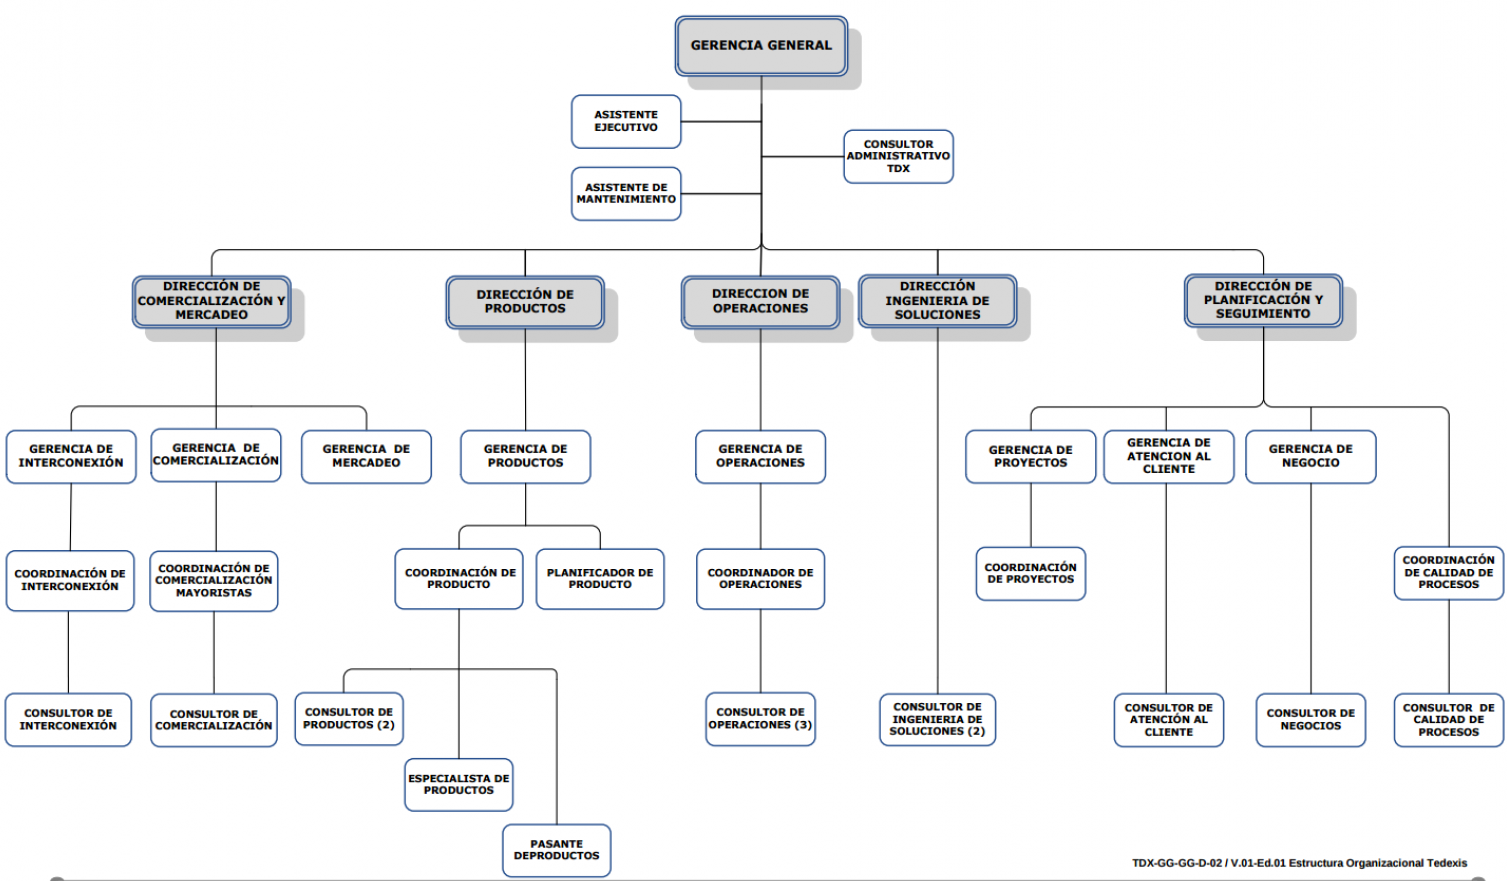
\includegraphics[scale=0.3,type=png,ext=.png,read=.png]{imagenes/organigrama} \\
  \caption{Estructura Organizacional de Tedexis}
  \label{fig:estsyn}
\end{figure}


% Marco Teorico.
\chapter{Marco Teórico} \label{chap:Marco Teorico}

\vspace{5 mm}

	En este capítulo se exponen los conceptos fundamentales que sustentan el trabajo realizado, adicionalmente se explican las herramientas tecnológicas utilizadas para el desarrollo.
	
\section{Framework} \label{sect:Framework}
Un framework se define como un conjunto estandarizado de conceptos, prácticas
y criterios para enfrentar un tipo de problema particular. De igual manera
puede ser visto como un esqueleto o patrón para el desarrollo de una aplicación.\cite{FW}

\section{Servicio Web} \label{sect:Servicio Web}
Un servicio web es un conjunto de protocolos y estándares empleados para
intercambiar información entre aplicaciones web, no necesariamente escritas
en el mismo lenguaje de programación, ni alojadas en la misma plataforma
por lo que brinda versatilidad en el desarrollo. Algunos de los servicios web
mas utilizados son: XML (Extensible Markup Language), SOAP (Simple Object Access Protocol), REST (Representational State Transfer) entre otros. Los servicios web dentro de un framework, son generalmente utilizados para establecer comunicación entre el back-end y front-end del producto a desarrollar.\cite{SW}

\section{Transferencia de Estado Representacional} \label{sect:REST}
La Transferencia de Estado Representacional (REST), es un estilo de arquitectura
para sistemas distribuidos. Se apoya en el protocolo HTTP para definir
todas las operaciones que puede realizar, GET, POST, PUT y DELETE, que permiten
la comunicación entre el servicio y el cliente. Gracias a la arquitectura
desacoplada y versatilidad en la comunicación entre productor y consumidor,
la popularidad en la utilizacion de REST aumente considerablemente.\cite{REST}

\section{Patrón MVC} \label{sect:MVC}
Modelo-Vista-Controlador es un patrón de diseño que busca estructurar aplicaciones de manera modular.\cite{MVC} Para esto, se pueden apreciar tres componentes:
\begin{itemize}[noitemsep,nolistsep]
\item Modelo: Aqui se encuentra encapsulada la estructura y funcionalidad de la aplicacion.
\item Vista: Este componente representa la interfaz gráfica que es mostrada al usuario.
\item Controlador: El propósito del controlador es desacoplar el modelo de la vista. Define la forma en la que la aplicación reaccionará a la interacción con el usuario.\end{itemize}

\section{Hilos} \label{sect:Hilos}
Los hilos, también conocidos como \textit{Threads} es una forma de
realizar concurrencia, los distintos hilos de ejecución comparten una serie de recursos tales como el espacio de la memoria, los archivos abiertos, etc. Un hilo es simplemente una tarea que puede ser ejecutada al mismo tiempo con otra tarea.\cite{hilo}

\section{JavaScript} \label{sect:JS}
JavaScript es un lenguaje interpretado, orientado a objetos, débilmente tipado
y dinámico. Los objetos se crean añadiendo métodos y propiedades. Una vez se ha construido un objeto, puede usarse como modelo (o prototipo) para crear objetos similares.\cite{JS}


\section{AngularJS} \label{sect:AJS}
AngularJS es un framework estructural para aplicaciones web dinámicas. Su
uso permite la modularidad e independencia de Mediante el enlace de datos y la inyección de dependecias facilita muchísimo el trabajo de desarrolladores permitiendo que el codigo sea mucho mas simplificado y concreto. Funciona unicamente en el Front-End, lo que permite poder usar cualquier cosa en el Back-End sin que se vea afectado su funcionamiento. 

Un uso adecuado de este framework proporciona ventajas como reusabilidad, modularidad e independecia del servidor.\cite{ANG}

\section{MongoDB} \label{sect:MongoDB}
MongoDB es una base de datos NoSQL basada en esquemas, que gracias a su escalibilidad y agilidad permite que los esquemas puedan cambiar rápidamente a medida que las aplicaciones evolucionan, proporcionando siempre la funcionalidad que los desarrolladores esperan de las bases de datos tradicionales, tales como índices secundarios, un lenguaje completo de búsquedas y consistencia estricta.\cite{MDB}

\section{Bower} \label{sect:Bower}
Bower es un manejador de versiones que administra componentes que tienen HTML, CSS, JavaScript entre otros. Te permite instalar las dependencias con los paquetes necesarios.\cite{BW}

\section{NodeJS} \label{sect:NodeJS}
Es una plataforma desarrollada sobre V8 JavaScript Runtime, posee una arquitectura basada en un manejador de eventos capaz de realizar taréas asincronas en I/O, lo que lo hace eficiente para aplicaciones que manejan grandes cantidades de datos en tiempo real.\cite{NODE}

\section{NPM} \label{sect:NPM}
Node package manager, también conocido como NPM, es un manejador de paquetes o módulos que permite a los desarrolladores compartir soluciones. Con NPM se puede especificar la versión que se desea instalar y las dependencias necesarias.\cite{NPM}

\section{HTML} \label{sect:HTML}
El lenguaje de marcado de hipertexto (HyperText Markup Language) es el elemento de construcción más básico de una página web y se utiliza para crear y representar visualmente una página web.\cite{HTML}

\section{JSON} \label{sect:JSON}
JSON (JavaScript Object Notation) es un formato ligero de intercambio de datos. Es fácil de leer y escribir para humanos, como es de fácil de parsear y generar para computadoras\cite{Json}. Esta compuesto de dos estructuras:
\begin{itemize}[noitemsep,nolistsep]
\item Collecciones, que vienen en pares de nombre y valor
\item Lista ordenada de valores.
\end{itemize}

\section{JAVA} \label{sect:JAVA}
Java es un lenguaje de programación orientado a objetos. Su propósito es permitir que los desarrolladores de aplicaciones escriban el programa una vez y lo ejecuten en cualquier dispositivo.\cite{JV}

\section{Bitbucket} \label{sect:Bitbucket}
Bitbucket es controlador de versiones distribuido, que facilita el trabajo grupal y permite alojamiento web a todo tipo de proyectos. Este servicio está escrito en Python.\cite{BB}

\section{JAX-RS} \label{sect:JAX-RS}
JAX-RS también conocido como Java API for RESTful Web Services, es una API implementada en JAVA que proporciona los recursos necesarios para la creación de servicios web de acuerdo al estilo REST \cite{jar}.

\section{Jersey} \label{sect:Jersey}
Jersey para servicios web RESTful es un framework de código abierto de calidad que provee soporte para JAX-RS y sirve como una implementación de las referencias de JAX-RS. Jersey tiene su propio API con características adicionales y utilidades que ayudan aún más a simplificar el servicio REST y el desarrollo del cliente \cite{jersey}.



% Marco Metodologico.
\chapter{Marco Metodológico} \label{chap:Marco Metodologico}

\vspace{5 mm}

		Este capítulo describe la metodología de desarrollo utilizada durante el proyecto de pasantía. Para este proyecto se empleó la metodología ágil SCRUM, debido a que el departamento de producto, el equipo de desarrollo de software, utiliza esta metodología y es con la que han tenido mejores resultados.\cite{SCRUM} 
\newline
\newline
\indent En este proyecto de pasantía, el \textit{Product Owner} fue un consultor de producto y el \textit{Scrum Master} el coordinador de producto, ambos supervisados por la direcotra de productos. A continuación se presentan los componentes que forman parte de esta metodología:
		
\section{Roles} \label{sect:Roles}
 Existen tres roles principales dentro del equipo de trabajo, cada rol posee un conjunto de actividades bien definidas que deben ser realizadas en un período de tiempo específico para que el proyecto pueda culminar de manera exitosa. Estos son los roles:
 
\subsection{Scrum Master} \label{sect:Scrum Master}
El Scrum Master, es responsable de asegurar que el proceso SCRUM sea entendido y aceptado por todos los miembros del equipo, esto se hace haciendo uso de las reglas, prácticas y teorías. Por otro lado, el Scrum Master actúa como mediador entre agentes externos y el equipo de desarrollo, de esta manera se minimiza los problemas que puedan existir con la interacción entre los mismos.\cite{SCRUM}
  
\subsection{Product Owner} \label{sect:Product Owner}
El Product Owner es responsable de maximizar el valor del producto en creación y el trabajo del equipo desarrollador o \textit{development team}, también tiene la visión del producto y trabaja en colaboración con usuarios, clientes y \textit{stakeholders}. El Product Owner es el único responsable de determinar cuales son las funcionalidades a crear en el \textit{product backlog} o pila del producto.\cite{SCRUM}

\subsection{Development Team} \label{sect:Development Team}
Es el equipo de trabajo que se encarga de llevar a cabo el diseño y desarrollo del software requerido. El equipo tiene la responsabilidad de cumplir con las historias del \textit{Product Backlog} para ir desarrollando paso a paso el producto, la manera en como se desarrollan estas historias es una decision tomada por el equipo. Por lo general consta de 3 a 9 personas.\cite{SCRUM}


\section{Eventos} \label{sect:Eventos}
Los eventos en la metodología Scrum son todas las reuniones utilizadas para crear regularidad y actualizar al equipo constantemente del estado del proyecto y las siguientes acciones que se deberian llevar a cabo. Todos estos eventos tienen un tiempo de duración y son aprovechados para revisar y adaptar cada una de las historias desarrolladas. Estos eventos son los siguientes:\cite{SCRUM}

\subsection{Sprint} \label{sect:Sprint}
El \textit{Sprint} es el corazón del \textit{Scrum}, es un período de tiempo donde se desarrollan ciertas historias propuestas en el \textit{Sprint Backlog} y se entrega un producto funcional. Es recomendado que la duración de los sprints sea constante y definida por el equipo de desarrollo en base a su experecia. Un nuevo \textit{Sprint} comienza inmediatamente despues de concluir uno.

\subsection{Sprint Planning} \label{sect:Sprint Planning}
\textit{Sprint Planning}, es la reunión que se realiza al inicio de cada \textit{Sprint} en la que se determinará que historias serán realizadas. El Product Owner, como se mencionó anteriormente, es el encargado de definir las historias y organizarlas según su prioridad, seguidamente el equipo de desarrollo determina las historias que pueden desarrollar.\cite{SCRUM}

\subsection{Daily Sprint Meeting} \label{sect:Daily Sprint Meeting}
Reunión de máximo 15 minutos diaria que sirve para sincronizar y actualizar el plan de actividades para las siguientes 24 horas de desarrollo. Esta reunión se realiza todos los dias y cada miembro resume lo que hizo el día anterior, como le va en el día y que problemas ha presentado.\cite{SCRUM}

\subsection{Sprint Review} \label{sect:Sprint Review}
Se lleva acabo al final de cada \textit{Sprint}, donde se muestran los avances realizados en el producto. Dichos avances son presentados al \textit{Product Owner} y todos los demás interesados (pueden estar presentes clientes finales). 

\subsection{Sprint Retrospective} \label{sect:Sprint Retrospective}
Esta reunión sirve para reflexionar sobre el último Sprint realizado y sirve para inspeccionar los problemas que se tuvieron y buscar una manera de solucionarlos en los sprints venideros. Tiene un maximo de duración de 3 horas.\cite{SCRUM}

\section{Artefactos} \label{sect:Artefactos}
Los artefactos de SCRUM representan trabajo o valor de diversas formas que son útiles para brindar transparencia para la inspección y adaptación. Estos artefactos están diseñados para maximizar el entendimiento de la información.\cite{SCRUM}

\subsection{Product Backlog} \label{sect:Product Backlog}
Product backlog o pila del producto es una lista ordenada de todas las historias que pueden ser necesarias para el producto, con descripciones detalladas y sus prioridades de todos los requisitos funcionales y no funcionales. Esta lista es dinámica y pública para todos los involucrados en el proyecto. La pila del producto es creada por el \textit{Product Owner} durante el \textit{Sprint Planning}. \cite{SCRUM}

\subsection{Sprint Backlog} \label{sect:Sprint Backlog}
Es un documento detallado por parte del equipo de desarrollo, donde
se predicen las actividades necesarias a desarrollar en el siguiente
\textit{sprint} para dar como terminadas ciertas taréas.\cite{SCRUM}

 % Marco Teorico.
\chapter{Desarrollo de la aplicación} \label{chap:Desarollo de la aplicacion}

\vspace{5 mm}

    Este capítulo describe el desarrollo completo del sistema empleando la metodología \textit{Scrum}. Se mostrarán los 12 \textit{Sprints} que corresponden a las siguientes fases: análisis y especificación de requerimientos, diseño e implementación. De igual manera, se describen los artefactos generados, actividades realizadas y soluciones a problemas presentados durante el desarrollo de cada \textit{Sprint}. A continuación se muestra en la tabla \ref{table:durSprint} la distribución del tiempo de cada \textit{Sprint}.
% \indent En la tabla \ref{table:durSprint}, se indica la distribución del tiempo que tomó cada Sprint para su realización.

 \begin{table}[H]
 \centering
 \begin{tabular}{p{2cm} p{8cm} p{3cm}} 
 \hline
 Sprint & Nombre & Duración Semanas \\ [0.5ex] 
 \hline\hline
 1 & Familiarizarse con la empresa & 2 \\ 
 \hline
 2 & Levantamiento de información & 1 \\
 \hline
 3 & Desarrollo de documentación & 1 \\
 \hline
 4 & Selección de tecnologías & 1 \\
 \hline
 5 & Desarrollo del back-end & 2 \\ 
 \hline
 6 & Autenticación & 2 \\ 
 \hline
 7 & Inicio del desarrollo de Reportes por Empresa & 3 \\ 
 \hline
 8 & Fin del desarrollo de Reportes por Empresa & 2 \\ 
 \hline
 9 & Desarrollo de Reportes por Pasaporte & 1 \\ 
 \hline
 10 & Desarrollo de ultimas vistas del front-end & 1 \\ 
 \hline
 11 & Pruebas por el personal de la empresa & 2 \\ 
 \hline
 12 & Redacción del libro de pasantias & 2 \\ [1ex]
 \hline
\end{tabular}
\footnotesize \caption{Tabla de duración de Sprints}
\label{table:durSprint}
\end{table}

%%%%%%%%%%%%%%%%%%%%%%%%%%%%%%
 
\section{Familiarizarse con la empresa} \label{sect:Familiarizarse con la empresa}

\subsection{Objetivos}
\begin{itemize}[noitemsep,nolistsep]
\item Integración y conocimiento general de la empresa Tedexis, modelo de negocio y lugar de trabajo. 
\end{itemize}

\subsection{Actividades}

\subsubsection{Familiarizarse con la empresa tedexis y el modelo de negocios empleado}
\indent Desde el año 2000, Tedexis ofrece servicios de alta calidad para que las empresas accedan fácilmente a la tecnología SMS. Las empresas tienen necesidades específicas para integrar el envío de SMS, ya sea para la comunicación interna entre sus empleados, como con sus clientes para el envío masivo de SMS.
\newline
\newline
\indent Tedexis ha desarrollado un \textit{Gateway} transaccional para el manejo de SMS llamado Mercurio que ofrece la posibilidad de integrarse con todos los proveedores de telecomunicaciones móviles de América Latina, vea la figura \ref{fig:tdx}.

\begin{figure}[ht]
  \centering
  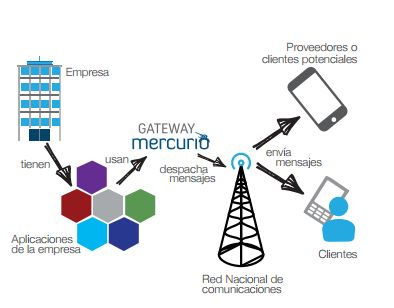
\includegraphics[scale=0.75,type=png,ext=.jpeg,read=.jpeg]{imagenes/tdx2} \\
  \caption{Tedexis}
  \label{fig:tdx}
\end{figure}
\pagebreak

\indent Los SMS se pueden clasificar como MO o MT dependiendo de su origen, como podemos ver en el gráfico \ref{fig:tdx1}. Si el mensaje es enviado por el usuario se le llama un mensaje MO y a la respuesta a este mensaje proveniente de una aplicación, se le llama MT, como por ejemplo la consulta de saldo por parte de un usuario es un MO, y la respuesta con el saldo es un MT.

\begin{figure}[ht]
  \centering
  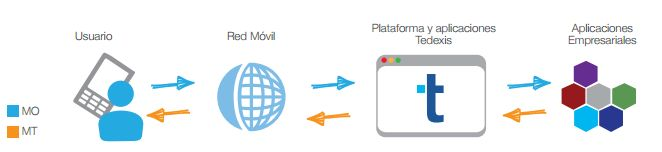
\includegraphics[scale=0.65,type=png,ext=.jpeg,read=.jpeg]{imagenes/tdx} \\
  \caption{Vista ejemplo de MO y MT}
  \label{fig:tdx1}
\end{figure}

\subsubsection{Analizar el modelo de datos local, de la plataforma y demás fuentes de datos de la aplicación}
\indent Inicialmente se realizaron dos reuniones donde se mostraron el modelo de datos actual que posee la empresa Tedexis en su plataforma Mercurio. Mercurio es una puerta de enlace de manejo de SMS, capaz de integrar diferentes proveedores nacionales e internacionales en la lógica de intercambio de los mensajes de texto. La mayoría de las bases de datos están en PostgreSQL, pero poseen como proyecto la migración de dichas bases de datos a MongoDB.
\newline
\newline
\indent De igual manera se recibieron tres clases donde se mostro parte del código que se utiliza como estándar para el desarrollo de aplicaciones en java dentro de Tedexis. Entre el código mostrado estaban librerías para conexiones a bases de datos PQSL las cuales tuvieron que ser adaptadas para el funcionamiento con MongoDB; librería para el uso de \textit{Logs} o registros; y librerías para el uso de MQ (\textit{Message queue}) las cuales no fueron utilizadas en este proyecto de pasantias.
\newline
\newline
\indent Estas reuniones fueron realizadas con el Scrum Master, quien realizó la mayoría de las explicaciones y un miembro del área de dirección de productos de Tedexis, quien expuso los conceptos sobre MongoDB.

%%%%%%%%%%%%%%%%%%%%%%%%%%%%

\section{Levantamiento de información} \label{sect:Levantamiento de informacion}

\subsection{Objetivos}
\begin{itemize}[noitemsep,nolistsep]
\item Definir reportes y funcionalidades a desarrollar. 
\end{itemize}

\subsection{Actividades}

\subsubsection{Obtener los reportes que genera el sistema y son usados por los clientes de Tedexis}

\indent Actualmente existe una versión de TID en producción, de la cual se tomaron los reportes minimos que debería poseer la segunda versión del sistema (TIID), por lo que se tomaron los reportes existentes como el alcance mínimo de la nueva versión. Los reportes fueron divididos en dos categorías: Reporte por empresa y reporte por pasaporte.
\newline
\newline
\indent Reporte por empresa muestra diferentes tipos de reportes referente a la empresa asociada al usuario, dichos reportes son: Evolución de tráfico de mensajes total enviados tanto por día como por hora por la empresa en un rango de tiempo, pasaportes asociados a la empresa, distribución de los mensajes enviados por las operadoras asociadas, campañas de mensajería masiva y top de empresas asociadas según la cantidad de mensajes que hallan enviado.
\newline
\newline
\indent Reporte por pasaporte muestra los reportes referente a los pasaportes asociados al usuario como individuo, dichos reportes son: Evolución de tráfico de mensajes enviados tanto por día como por hora y distribución de mensajes enviados por operadoras. La consulta de la información de todos los reportes se realiza eligiendo un rango de fechas especifico.

\subsubsection{Definir las opciones que existen por cada reporte generado por el sistema e identificar los servicios que son ofrecidos por la interfaz}

\indent Al tener definidos los reportes a implementar, se decidió que la información debería mostrarse en tablas, de igual manera, se definieron los campos especificos que debían mostrarse por cada reporte en dichas tablas y los tipos de gráficos que deberían mostrarse según el tipo de reporte los cuales fueron: Gráficos de líneas y barras en los reportes de evolución de tráfico; gráfico de torta en reporte de operadoras y top empresas.
\newline
\newline
\indent Posteriormente, se concretó que los datos mostrados en las tablas deberían poder ser exportados por el usuario en formato csv, de igual manera, la tablas deberían poseer algún mecanismo de búsqueda y reorganización de los datos mostrados tanto por campos individuales como de forma global.

\subsubsection{Obtener los roles disponibles y los privilegios asociados}

\indent En la versión actual del sistema, los usuarios son gestionados por un sistema externo a TID por lo que se decidió crear un módulo de usuarios dentro de TIID. Inicialmente se propone que dentro de TIID el usuario administrador sea quien pueda crear y editar los usuarios del sistema, teniendose como perfiles: Tedexis (administrador) y canales (usuario regular). Con la diferencia de que el perfil tedexis posee acceso a todo el sistema, mientras que el perfil canales tiene restringidas ciertas vistas.

% %%%%%%%%%%%%%%%%%%%%%%%%%%%%

\section{Desarrollo de documentación} \label{sect:Desarrollo de documentacin}

\subsection{Objetivos}
\begin{itemize}[noitemsep,nolistsep]
\item Diseño de la solución global a implementar, parte 1. 
\end{itemize}

\subsection{Actividades}

\subsubsection{Creación de documentos inciales}
\indent Siguiendo los estandares de Tedexis, primero fue solicitado crear un documento de los casos de usos del sistema, utilizando una plantilla proporsionada por la empresa. Teniendo como versión final el siguiente diagrama \ref{fig:cdu}. Donde se muestran las funcionalidades que tiene acceso el usuario como son, autenticación, soporte y los diferentes reportes.
\pagebreak
\begin{figure}[ht]
  \centering
  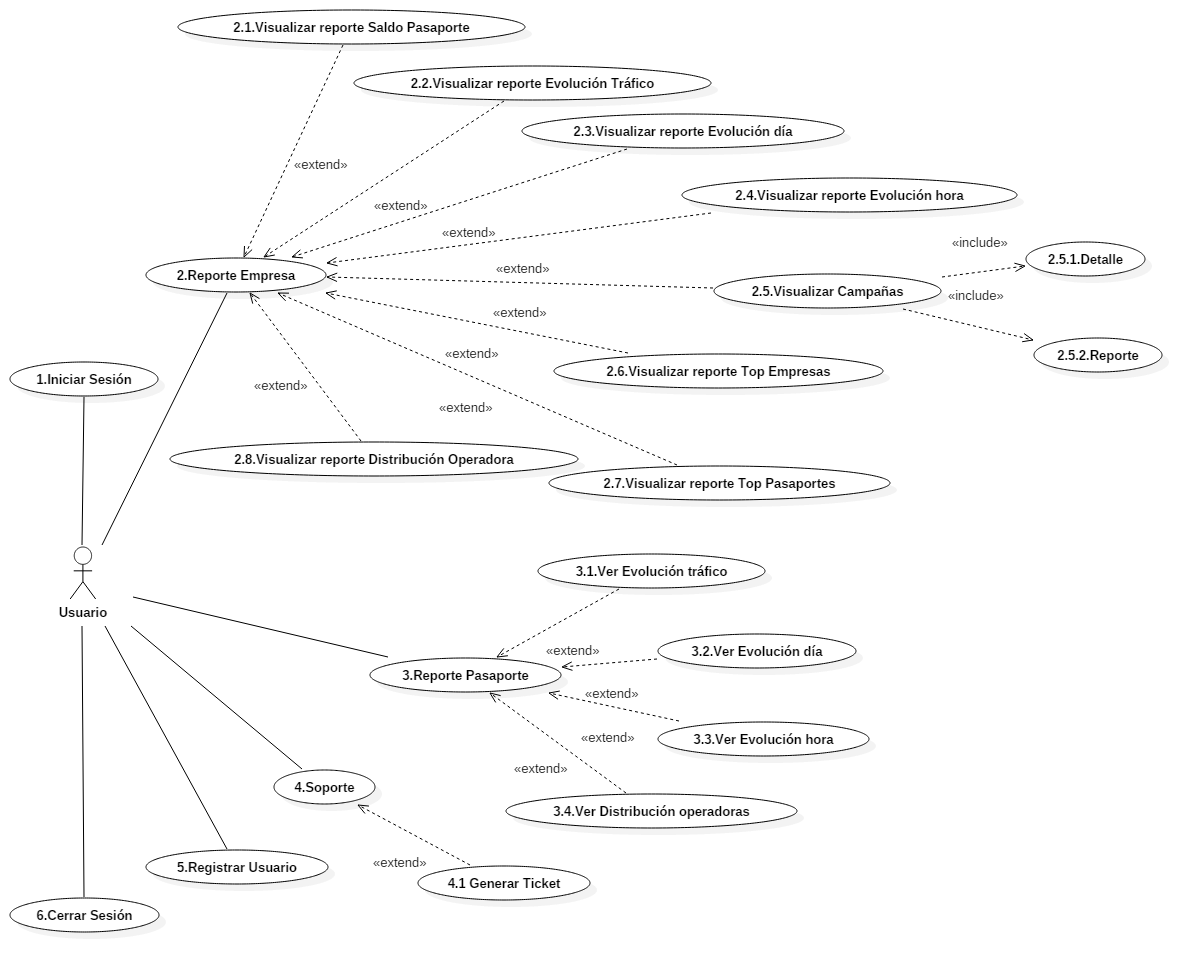
\includegraphics[scale=0.42,type=png,ext=.png,read=.png]{imagenes/cdu}
  \caption{Diagrama de casos de uso.}
  \label{fig:cdu}
\end{figure}
\newline
\newline
\indent Seguidamente, el \textit{Product Owner} solicitó la elabolarición de tres documentos: diccionario de datos, donde se muestra una versión inicial de la base de datos del sistema, dicha base de datos se implementó utilizando el manejador MongoDB por motivos de investigación de la empresa; el documento de vistas del sistema, en el que se muestran vistas tentativas de la interfaz del sistema; por último el documento de diagrama de despligue el cual muestra dicho diagrama, elaborado siguiendo el prototipo especificado por la empresa, como se puede apreciar en la figura \ref{fig:ddd}. 
\pagebreak
\begin{figure}[ht]
  \centering
  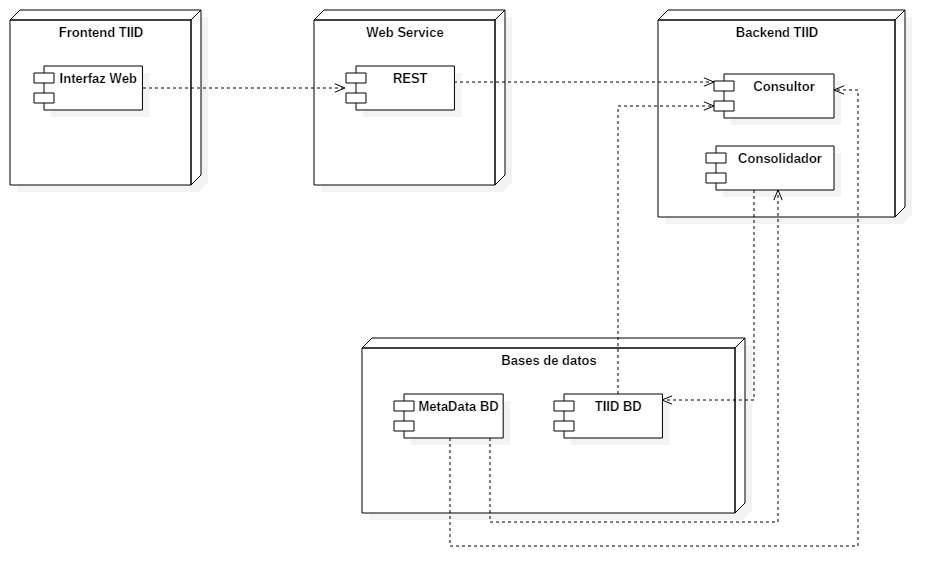
\includegraphics[scale=0.50,type=png,ext=.png,read=.png]{imagenes/ddd}
  \caption{Diagrama de despligue.}
  \label{fig:ddd}
\end{figure}

\indent Este diagrama de despliegue \ref{fig:ddd} muestra de forma global como esta organizado el sistema, divido en front-end, desarrollado con el \textit{framework} AngularJS, servicio web desarrollados utilizando la arquitectura REST y back-end. El back-end posee dos apartados: el consolidador, que resume la información proveniente de una base de datos con información detalla, con el fin de optimizar los tiempos de respuesta en las consultas; y el consultor, el cual se encarga de realizar las consultas, provenientes de los servicios web, contra las bases de datos. Las bases de datos consultadas son: MetaDataDB de la que se utiliza la colección RTD (Reporte de tráfico detallado), la cual posee información detallada de todos los mensajes enviados por la empresa. Esta base de datos pertenece a otro sistema ajeno a TIID, la cual es utilizada cuando se activa el consolidador en el back-end ó cuando el cliente requiere reportes del día actual; y la base de datos TIID, la cual posee la información consolidad por cada usuario.

% %%%%%%%%%%%%%%%%%%%%%%%%%%%%
\section{Selección de tecnologías} \label{sect:Seleccion de tecnologias}

\subsection{Objetivos}
\begin{itemize}[noitemsep,nolistsep]
\item Diseño de la solución global a implementar, parte 2. 
\end{itemize}

\subsection{Actividades}

\subsubsection{Selección de frameworks de desarrollo}
\indent Para el desarrollo del sistema, se estableció desde un principio que el Back-End debía ser desarrollado enteramente en java utilizando el IDE Netbeans, ya que es el lenguaje de programación y el entorno de desarrollo integrado mayormente utilizados dentro de Tedexis. De igual manera el desarrollo del servicio REST cumplió el mismo estandar.
\newline
\newline
\indent Para el desarrollo del Front-End se probaron diferentes herramientas. El personal de Tedexis tenía mayor preferencia por frameworks de desarrollo basados en java por lo que se probaron Sprint, Play y Grails, haciendo simples implementaciones \textit{Hola Mundo} con cada uno, sin embargo, se decidió utilizar AngularJS por la gran cantidad de documentación disponible y experiencia por parte del pasante con la herramienta. Con la utilización de dicho framework se lograron buenas prácticas de programación utilizando el patrón MVC (Modelo Vista Controlador), la arquitectura REST, el manejador de bases de datos MongoDB y el controlador de versiones Bitbucket.  

% %%%%%%%%%%%%%%%%%%%%%%%%%%%%

\section{Desarrollo del back-end} \label{sect:Desarrollo del back-end}

\subsection{Objetivos}
\begin{itemize}[noitemsep,nolistsep]
\item Desarrollo del back-end. 
\end{itemize}

\subsection{Actividades}
\indent Este \textit{sprint} muestra el desarrollo del back-end del sistema, el cual fue desarrollado enteramente en java, creadose como un proyecto tipo \textit{Java Application} en \textit{Netbeans} para tomar tu estructura de organización de archivos.
\newline
\newline
\indent TIID tiene como función principal mostrar diferentes reportes a los usuarios sobre su uso del servicio de mensajería que les provee la empresa Tedexis, por lo cual tiene que manejar una gran cantidad de datos provenientes de la base de datos de la plataforma Mercurio. Esta plataforma consta de tres esquemas en PostgreSQL: Mercurio con seis tablas, DLR con doce tablas y Content con una tabla. Estos tres esquemas sirven como fuente de información para una base de datos en MongoDB, llamada MetaData la cual posee una colección que centraliza la información pertinente de los tres esquemas de la base de datos PostgresSQL. MetaData es una base de datos ajena a TIID, por lo que fue simulada durante el desarollo del sistema, de igual manera, posee una colección que tiene por nombre RTD (Reporte de Tráfico Detallado), quien es la principal fuente de información que utiliza TIID para generar todos sus reportes.
\newline
\newline
\indent Ya que la colección RTD tiene la información centralizada de todos los esquemas de Mercurio, posee información que en muchos casos no son pertinentes para los reportes de TIID, por lo cual se crearon dos hilos que consolidan la información necesaria para el sistema. 

\subsubsection{Diseño y creación de la base de datos}
\indent Se tomó como manejador de bases de datos MongoDB, debido a que Tedexis tiene futuros proyectos la migración de sus bases de datos actuales de PostgreSQL a MongoDB por la mayor velocidad en el manejo de grandes cantidades de datos, por lo que se decidió investigar con el proyecto de pasantía.
\newline
\newline
\indent La base de datos de TIID consta de cinco colecciones, como se puede vizualizar en el dragrama \ref{fig:bd}, las cuales se muestran a continuación:
\begin{figure}[ht]
  \centering
  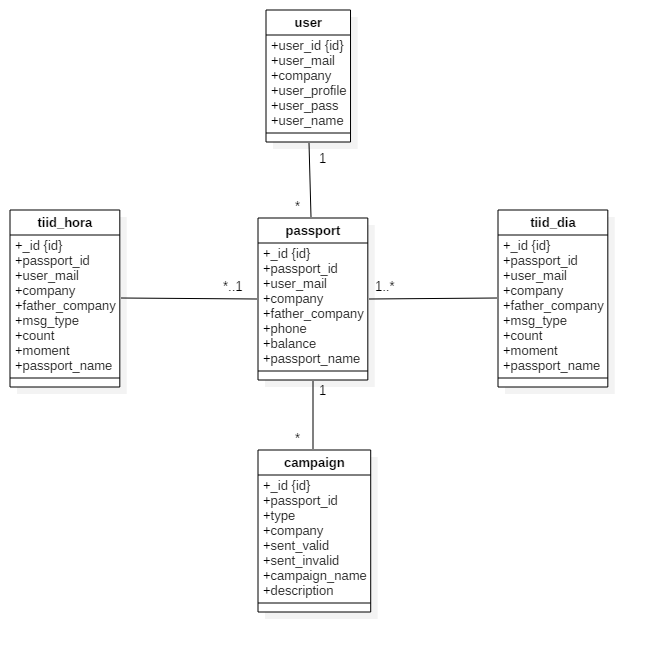
\includegraphics[scale=0.50,type=png,ext=.png,read=.png]{imagenes/bd}
  \caption{Diagrama de conceptual de base de datos.}
  \label{fig:bd}
\end{figure}

\begin{itemize}[noitemsep,nolistsep]
\item \textbf{user}: Almacena la infomación correspondiente a los usuarios de TIID. Posee los siguientes campos:
\begin{itemize}[noitemsep,nolistsep]
\item \textbf{user\_id}: identificación del usuario dentro de la colección. Ejemplo: Alejandro.
\item \textbf{user\_name}: nombre del usuario. Ejemplo: Alejandro.
\item \textbf{user\_mail}: correo electrónico del usuario. Ejemplo: alejandro@gmail.com
\item \textbf{company}: corresponde a la compañía donde pertenece el usuario. Ejemplo: Tedexis.
\item \textbf{user\_profile}: representa el perfil o privilegio del usuario. TIID posee dos perfiles, Tedexis (Administrador) y Canales. Ejemplo: Tedexis.
\item \textbf{user\_pass}: contraseña del usuario.
\end{itemize} 
\item \textbf{passport}: Almacena la información de los pasaportes asociados a los usuarios de TIID. Los pasasportes son el equivalente a la identificación del usuario.\begin{itemize}[noitemsep,nolistsep]
\item \textbf{\_id}: identificación del pasaporte dentro de la colección. Creado automaticamente por el manejador.
\item \textbf{passport\_id}: identificación de los pasaportes. Ejemplo: 42.
\item \textbf{passport\_name}: nombre del pasaporte. Ejemplo: AlejandroLunch
\item \textbf{user\_mail}: correo electrónico del usuario que le pertenece dicho pasaporte. Ejemplo: alejandro@gmail.com.
\item \textbf{company}: nombre de la compañía asociada al pasaporte. Ejemplo: Banco de Venezuela.
\item \textbf{father\_company}: nombre de la empresa padre de la compañía asociada al pasaporte. Ejemplo: Tedexis.
\item \textbf{phone}: número de contacto del propietario del pasaporte. Ejemplo: +584149322879.
\item \textbf{balance}: saldo disponible del pasaporte. Ejemplo: 1000.
\end{itemize} 
\item \textbf{campaign}: Almacena los datos de las campañas de mensajería asociadas a las empresas.
\begin{itemize}[noitemsep,nolistsep]
\item \textbf{\_id}: identificación de la campaña dentro de la colección. Creado automaticamente por el manejador.
\item \textbf{campaign\_name}: nombre de la campaña. Ejemplo: Navidad 2016.
\item \textbf{descriptio}: descripción de la campaña. Ejemplo: Promociones para la época decembrina 2016.
\item \textbf{type}: tipo de mensajes enviados en la campaña. Ejemplo: MT.
\item \textbf{company}: nombre de la compañía a la que pertenece la campaña. Ejemplo: Banco de Venezuela.
\item \textbf{sent\_valid}: número de mensajes enviados exitosamente. Ejemplo: 42.
\item \textbf{sent\_invalid}: número de mensajes que no pudieron ser enviados. Ejemplo: 9.
\end{itemize} 
\item \textbf{tiid\_hora}: Almacena la información por hora, pertinente para TIID, de la colección RTD de la base de datos MetaData.
\begin{itemize}[noitemsep,nolistsep]
\item \textbf{\_id}: identificación del registro dentro de la colección. Creado automaticamente por el manejador.
\item \textbf{passport\_id}: identificación del pasaporte que envió los mensajes. Ejemplo: 42.
\item \textbf{passport\_name}: nombre del pasaporte que envió los mensajes. Ejemplo: AlejandroLunch
\item \textbf{user\_mail}: correo electrónico del usuario que le pertenece dicho pasaporte. Ejemplo: alejandro@gmail.com.
\item \textbf{company}: nombre de la compañía asociada al pasaporte. Ejemplo: Banco de Venezuela.
\item \textbf{father\_company}: nombre de la empresa padre de la compañía asociada al pasaporte. Ejemplo: Tedexis.
\item \textbf{msg\_type}: tipo agrupado de los mensajes enviados. Ejemplo: MO.
\item \textbf{count}: cantidad de mensajes enviados a cierta fecha y hora. Ejemplo: 100.
\item \textbf{moment}: fecha y hora a que fueron enviados los mensajes. Ejemplo: 11-13-2016 16:00:53.
\end{itemize} 
\item \textbf{tiid\_día}: Almacena la información por día, pertinente para TIID, de la colección RTD de la base de datos MetaData.
\begin{itemize}[noitemsep,nolistsep]
\item \textbf{\_id}: identificación del registro dentro de la colección. Creado automaticamente por el manejador.
\item \textbf{passport\_id}: identificación del pasaporte que envió los mensajes. Ejemplo: 42.
\item \textbf{passport\_name}: nombre del pasaporte que envió los mensajes. Ejemplo: AlejandroLunch
\item \textbf{user\_mail}: correo electrónico del usuario que le pertenece dicho pasaporte. Ejemplo: alejandro@gmail.com.
\item \textbf{company}: nombre de la compañía asociada al pasaporte. Ejemplo: Banco de Venezuela.
\item \textbf{father\_company}: nombre de la empresa padre de la compañía asociada al pasaporte. Ejemplo: Tedexis.
\item \textbf{msg\_type}: tipo agrupado de los mensajes enviados. Ejemplo: MO.
\item \textbf{count}: cantidad de mensajes enviados a cierta fecha sin hora. Ejemplo: 100.
\item \textbf{moment}: fecha sin hora a la que fueron enviados los mensajes. Ejemplo: 11-13-2016.
\end{itemize} 
\end{itemize}

\subsubsection{Creación de hilos consolidadores de información}
\indent El sistema TIID se alimenta de los datos proveniente de la colección RTD, como fue antes mencionado, pero dicha colección posee mucha información no relevante para el sistema lo que ocasiona tiempo de respuestas muy largos y desesperación por parte de los usuarios al consultar su información. Por lo que para optimizar la experiencia del usuario, mejorar las consultas de bases de datos y poseer tiempos cortos de respuesta al momento de la carga de datos en el front-end del sistema, se decidió poseer la mayor cantidad de información procesada dentro de la base de datos de TIID.
\newline
\newline
\indent Para la consolidación de los datos de RTD, se crearon dos hilos:
\begin{itemize}[noitemsep,nolistsep]
\item \textbf{ThreadDayConsolidator}: esta clase fue creada como extensión de la clase \textit{Thread} de java, lo que permite redefinir el método \textit{run} para luego instanciar la clase y poner en ejecución el hilo con el método \textit{start}. Este hilo lo que hace es recorrer la colección \textit{passport} antes mencionada y por cada pasaporte totaliza la cantidad de mensajes MO, MT y MR enviados por día, mostrados en la colección RTD. Esta clase se apoya en una clase llamada \textit{Mongo} la cual a partir de un archivo de propiedades proporcionado, realiza las conexiones a las bases de datos MongoDB.
\item \textbf{ThreadHourConsolidator}: esta clase es análoga a la clase \textit{ThreadDayConsolidator} solo que totaliza los mensajes por hora en vez de por día. Es importante mencionar que ambos hilos se activan una vez por día y consolidan los datos correspondiente al día anterior, por lo que si se realizan consultas del día actual, dichas consultas se llevan acabo directo en colección RTD.
\end{itemize}

\subsubsection{Pruebas}
\indent Para las prueba de esta sección, primero se creó la bases de datos TIID en MongoDB con la colección \textit{passport} y luego se simuló la colección RTD de la base de datos MetaData. Ambas fueron llenadas mediante el comando \textit{mongoimport} \cite{mimport} con datos generados de forma aleatoria. Se pusieron a prueba ambos hilos por separado, primero \textit{ThreadDayConsolidator} y luego \textit{ThreadHourConsolidador} probando primero con 100 entradas en la colección RTD y 10 en la colección \textit{passport}, realizando la consolidación de la información sin ningún inconveniente. Luego se aumentó la cantidad de datos con 100000 entradas en RTD y 200 en \textit{passport}, superando la prueba sin ningún inconveniente.
\newline
\newline
\indent De igual manera, se realizaron pruebas de borde donde se simuló la activación de los hilos a media noche (12:00 am ó 00:00:00), donde se encontraron algunos inconvenientes que no tomaba en cuenta los mensajes enviados justo a media noche pero fue solucionado con un ajuste en el rango de las fechas.
\newline
\newline
\indent Finalmente se hicieron pruebas de integración, donde se activaron los dos hilos al mismo tiempo, agregando desde 100 hasta 100000 datos en RTD y desde 10 hasta 200 en \textit{passport}, lo que fue superado sin ningún inconveniente. Dichas pruebas fueron mostradas y aprobadas tanto por el \textit{Product Owner} como el \textit{Scrum Master}.
% %%%%%%%%%%%%%%%%%%%%%%%%%%%%

\section{Autenticación} \label{sect:Autenticacion}

\subsection{Objetivos}
\begin{itemize}[noitemsep,nolistsep]
\item Desarrollo del módulo de autenticación. 
\end{itemize}

\subsection{Actividades}

\subsubsection{Creación del servicio Web RESTful}
\indent Para la creación del módulo de autenticación, primero se creó el servicio REST como un proyecto java utilizando Netbeans. Utilizando las herramientas proporcionadas por el entorno de desarrollo integrado, se instaló y configuró el servidor GlashFish 4.2, que es un servidor \textit{open source} para el desarrollo y despliegue de plataformas y tecnologías basadas en java. Al haber instalado el servidor, se procedió a instalar las librerías necesarias para poder invocar el API \textit{Jersey} quen proporcina los mecanismos indispensables para el desarrollo de los servicios REST.

\subsubsection{Autenticación del usuario}
\indent Al tener el proyecto REST creado, se procedió al desarollo del módulo de autenticación. Se utilizó un módulo basado en \textit{tokens}\cite{tokens} para AngularJS llamado \textit{Satellizer} igualmente \textit{open source}\cite{satellizer}. Con \textit{Satellizer} se logró implementar de forma sencilla el inicio de sesión, cierre de sesión y creación de usuarios para el sistema. En la creación de usuarios se puede elegir entre dos perfiles, Tedexis (administrados) y Canales (usuario regular), diferenciandoses en que el perfil Tedexis puede crear nuevos usuarios del sistema mientras que Canales no. Cabe destacar que \textit{Satellizer} permitió una fácil integración con en manejador MongoDB, se partió de un ejemplo desarrollado en java con el manejador H2 el cual fue posteriormente adaptado. A continuación se presentan las vistas del inicio de sesión \ref{fig:login} y creación de usuarios \ref{fig:signup}.
\begin{figure}[ht]
  \centering
  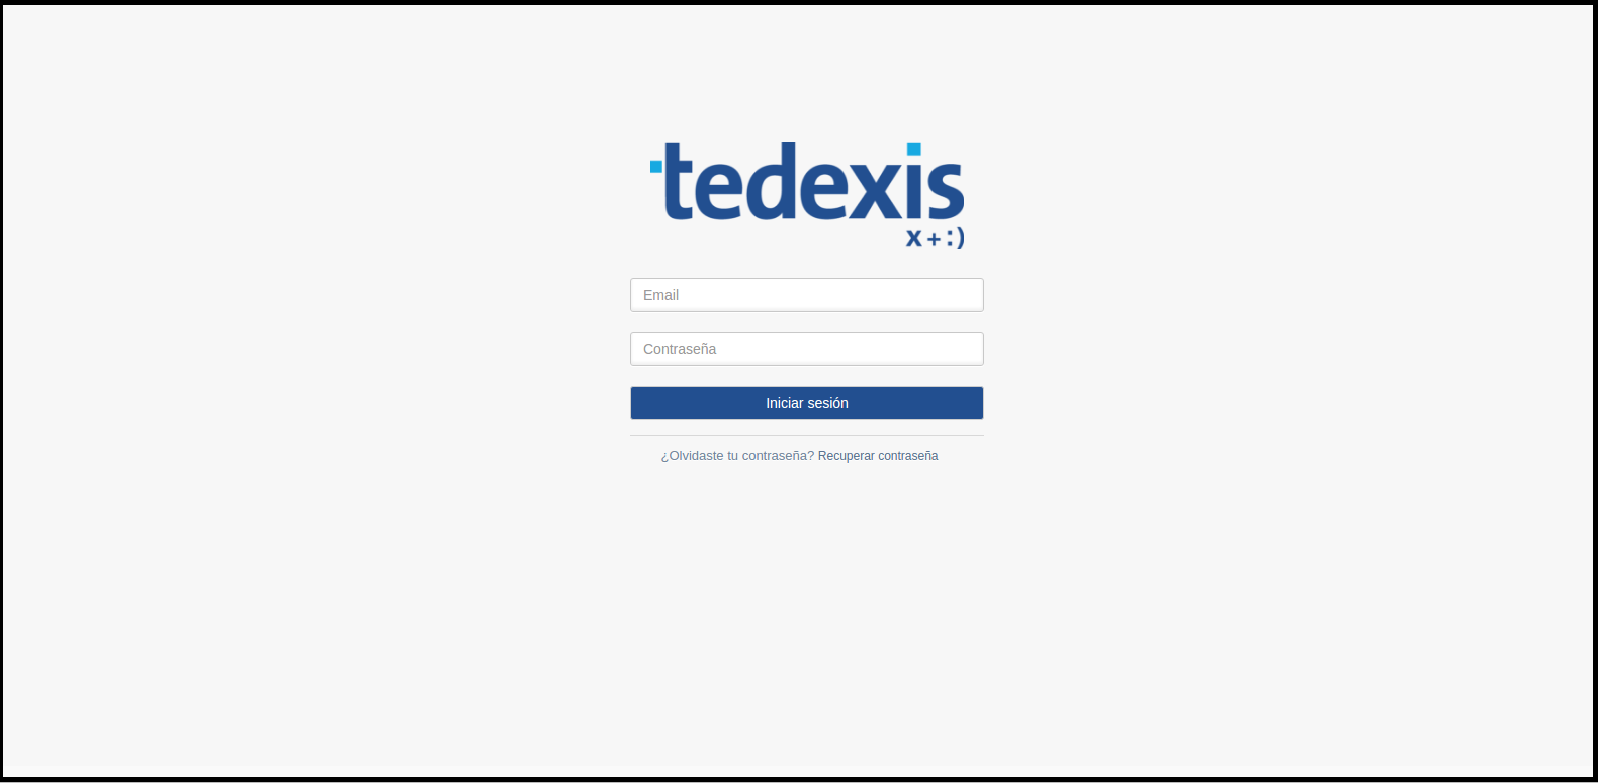
\includegraphics[scale=0.30,type=png,ext=.png,read=.png]{imagenes/login}
  \caption{Vista de inicio de sesión.}
  \label{fig:login}
\end{figure}

\begin{figure}[ht]
  \centering
  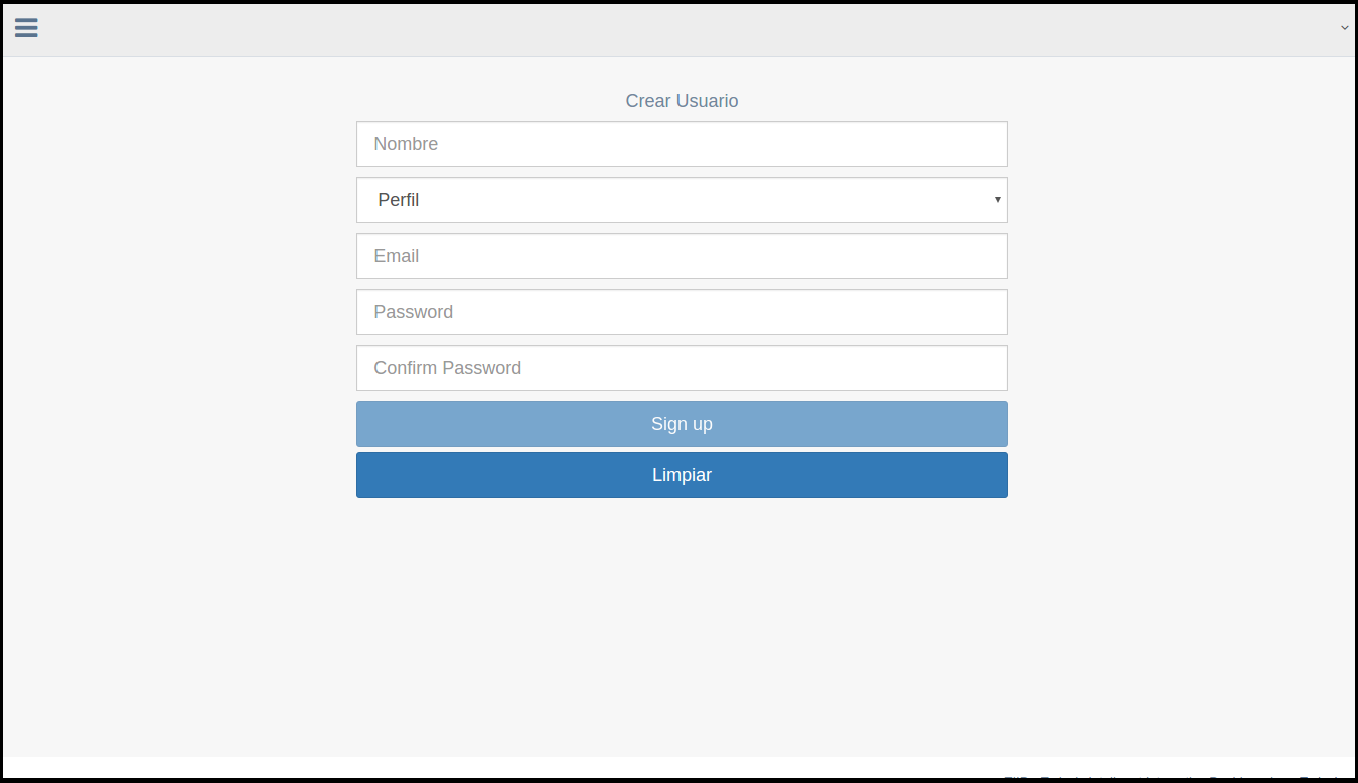
\includegraphics[scale=0.30,type=png,ext=.png,read=.png]{imagenes/signup}
  \caption{Vista de creación de usuario.}
  \label{fig:signup}
\end{figure}

\indent Posteriormente se desarrolló la recuperación de contraseña del usuario, el cual dado un correo electrónico verifica si existe en la base de datos y genera una nueva contraseña, la cual es enviada por correo electrónico al usuario.

\subsubsection{Pruebas}
\indent Al crear el proyecto RESTful se crearon métodos GETs de prueba para verificar que se estaba accediendo a la base de datos y las colecciones correspondientes. Seguidamente se integraron los métodos POSTs necesarios para el inicio de sesión y creación de usuario, con el front-end del sistema. Se realizaron distintas pruebas de creación de usuarios y de inicio de sesión donde surgieron las restricciones de no poder crear un nuevo usuario con un correo electrónico ya existente en el sistema y el cifrado de las contraseñas, lo cual se logró con una librería que proporsiona \textit{Satellizer}.

% %%%%%%%%%%%%%%%%%%%%%%%%%%%%

\section{Inicio del desarrollo de Reportes por Empresa} \label{sect:Inicio del desarrollo de Reportes por Empresa}

\subsection{Objetivos}
\begin{itemize}[noitemsep,nolistsep]
\item Desarrollo de reportes por empresa, parte 1. 
\end{itemize}

\subsection{Actividades}
\indent En este \textit{Sprint} se empezó con el desarrollo a fondo del front-end del sistema. El equipo de mercadeo de Tedexis proporsionó unas serie de documentos con los recursos visuales utilizados por la empresa, íconos, colores, logos, entre otros. y una plantilla llamada Gentelella \cite{gentelella}, la cual sirvió como base para el desarrollo de las vistas de TIID.

\subsubsection{Creación de vista Saldo Pasaporte}
\indent La vista inicial que se creó en el sistema, muestra una tabla con todos los pasaportes asociados al usuario cuya sesión esta activa, como se puede apreciar en figura \ref{fig:saldopasaporte}. En la creación de esta vista surgieron distintos problemas, ya que fue la primera tabla implementada combinando la librería proposionada por la plantilla Gentelella con los datos provenientes de la llamada de servicio RESTful. Dicha llamada es asincrona al momento de la carga de la página, lo que ocasionaba que en algunas ocasiones no se mostraran los datos, esto se resolvió utilizando promesas como cuerpo de las tablas al momento su creación.

\begin{figure}[ht]
  \centering
  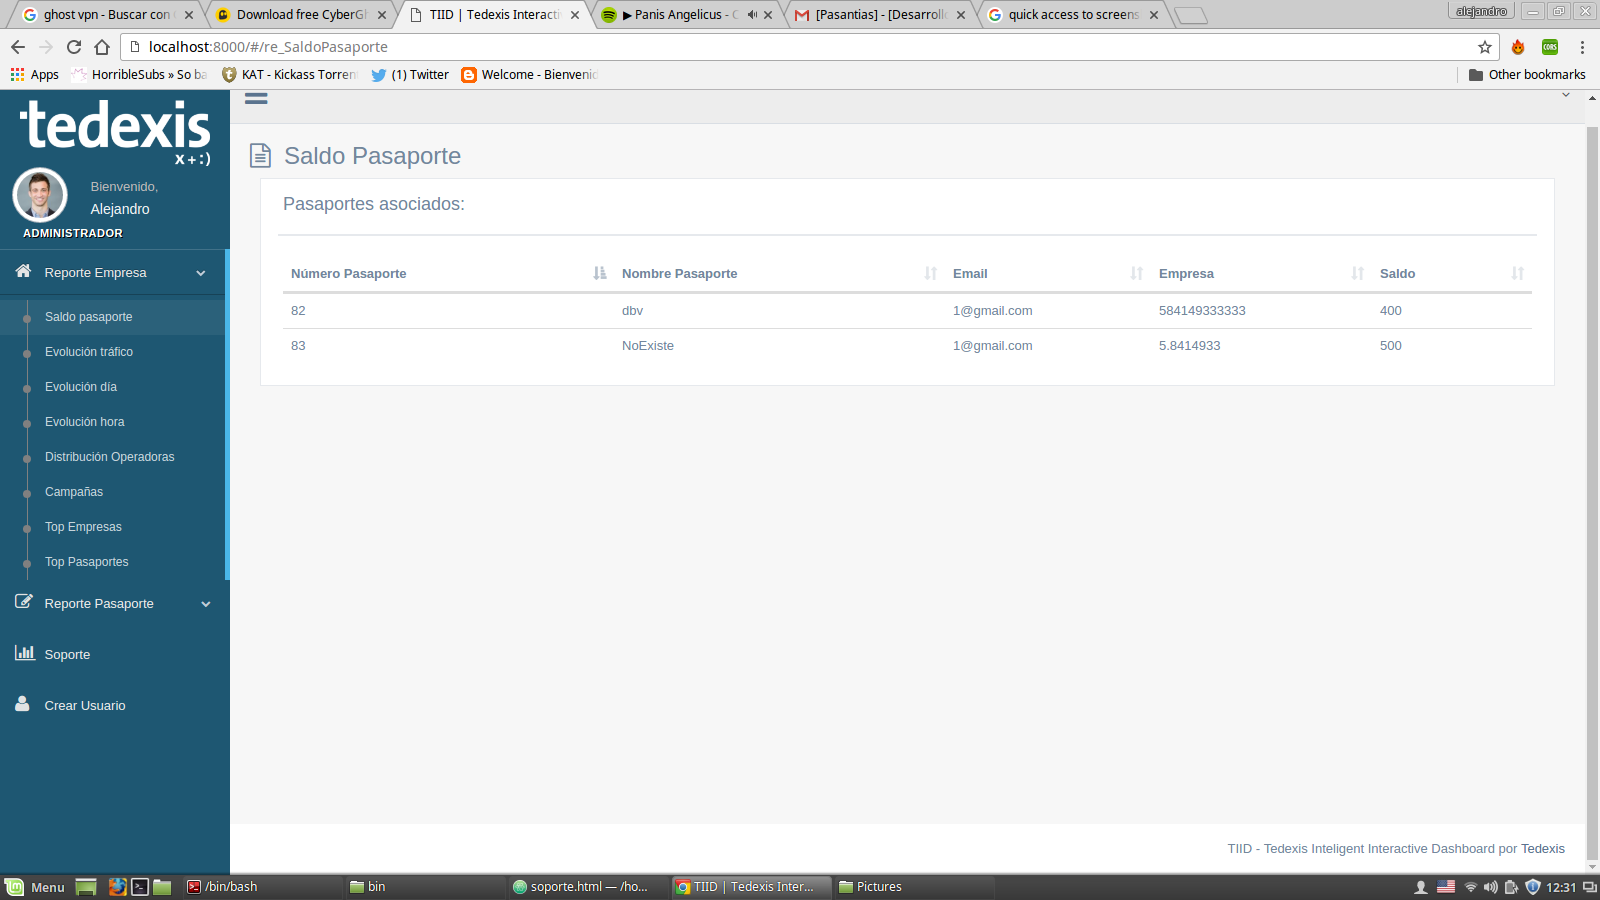
\includegraphics[scale=0.25,type=png,ext=.png,read=.png]{imagenes/saldopasaporte}
  \caption{Reporte Empresa: Saldo Pasaporte.}
  \label{fig:saldopasaporte}
\end{figure}

\subsubsection{Creación de vista Evolución del Tráfico}
\indent Esta vista muestra el reporte de mensajes tipo MT y MR enviados por día por la empresa asociada al usuario en un rango de tiempo específico, el usuario puede elegir dicho rango de tiempo mediante un \textit{widget} de calendario proporsionado y puede descargar tanto el gráfico mostrado en un una imagen png, como la información del reporte mostrada en la tabla en un archivo de formato csv. De igual manera, el usuario puede aplicar distintos filtros y métodos de búsqueda proposionados por las funcionalidades de la tabla. Vea la figura \ref{fig:reet}.

\begin{figure}[ht]
  \centering
  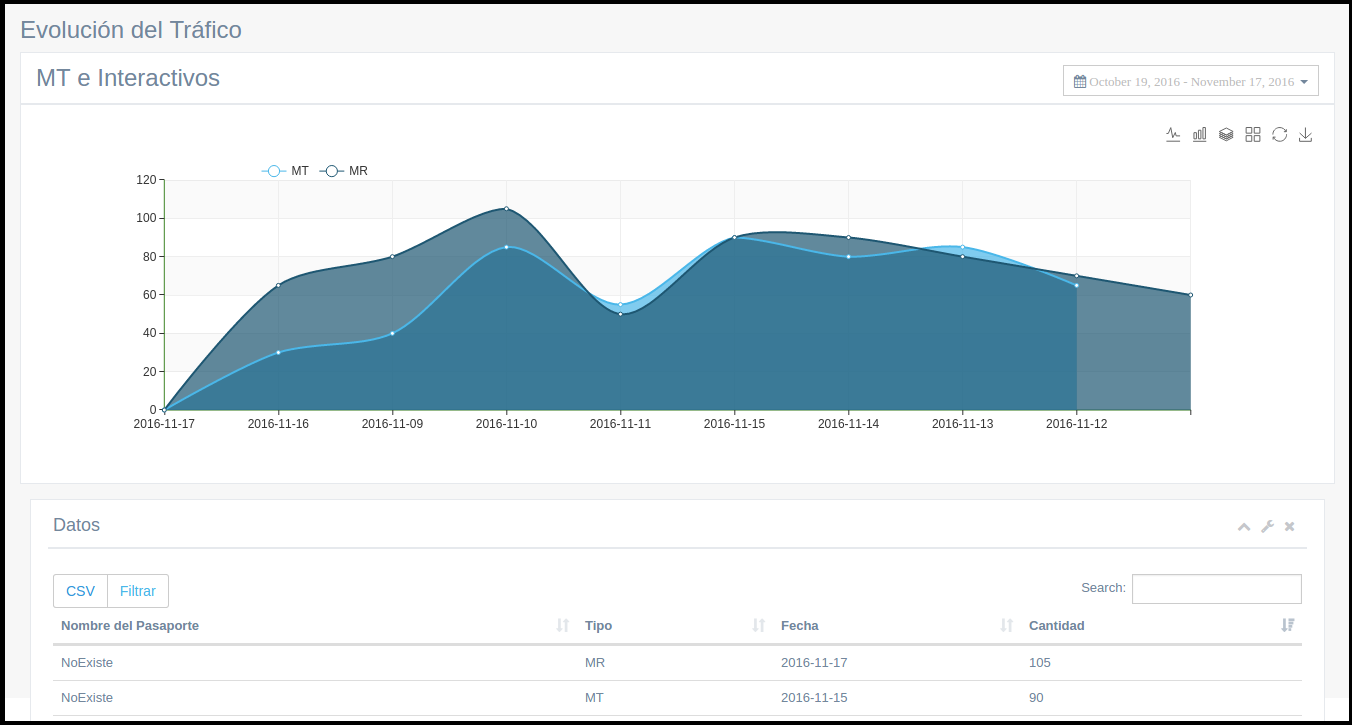
\includegraphics[scale=0.30,type=png,ext=.png,read=.png]{imagenes/reet}
  \caption{Reporte Empresa: Evolución del Tráfico.}
  \label{fig:reet}
\end{figure}

\indent Para el desarrollo de esta vista primero se crearon los servicios RESTful que consulta la información consolidada en la colección “tiid\_dia" de la base de datos de TIID tanto para el gráfico como la tabla. Luego se escribieron las funciones para generar el gráfico y la tabla, incorporando el rango de fechas proposionado por un \textit{widget} calendario.

\subsubsection{Creación de vistas Evolución Día y Evolución Hora}
\indent La vista \textit{Evolución Día} es análoga a la vista \textit{Evolución del Tráfico} solo que muestra la información consolidada por día de los mensajes tipo MT y MO, mostrada en la figura \ref{fig:reed}. En cambio la vista \textit{Evolución Hora} sigue la misma lógica que las dos anteriores pero consulta la información consolidad por hora de la colección “tiid\_hora", por lo que se crearon los servicios de consulta REST respectivos. La figura \ref{fig:reeh} muestra el reporte por hora.
% \pagebreak
\begin{figure}[ht]
  \centering
  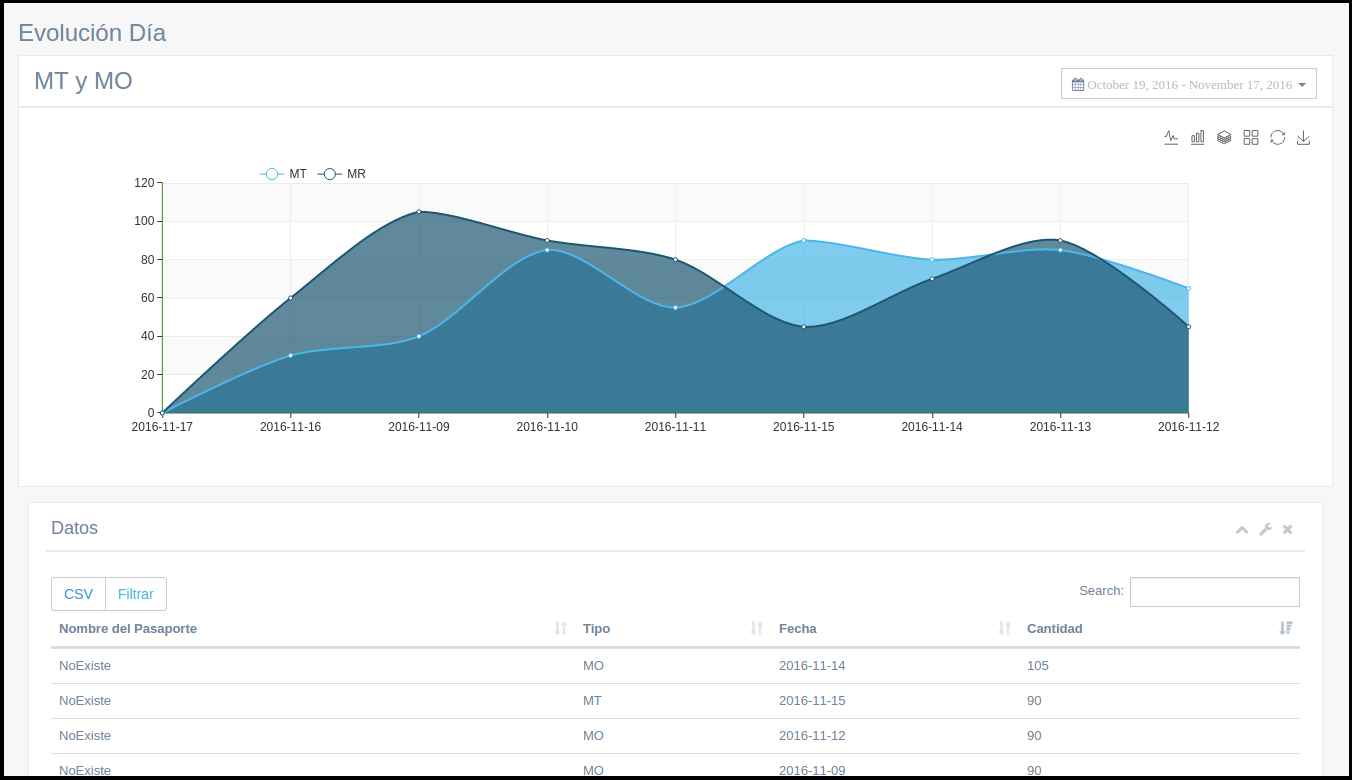
\includegraphics[scale=0.30,type=png,ext=.png,read=.png]{imagenes/reed}
  \caption{Reporte Empresa: Evolución Día.}
  \label{fig:reed}
\end{figure}

\begin{figure}[ht]
  \centering
  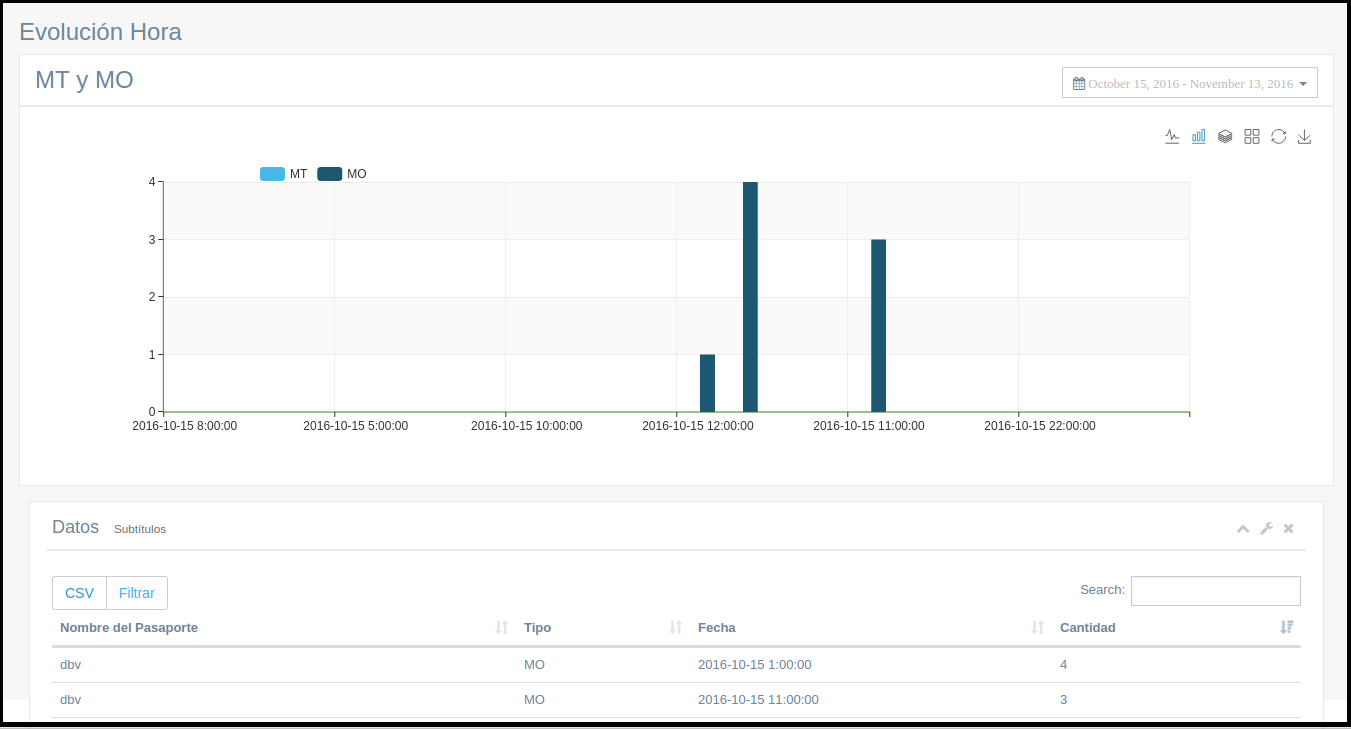
\includegraphics[scale=0.30,type=png,ext=.png,read=.png]{imagenes/reeh}
  \caption{Reporte Empresa: Evolución Hora.}
  \label{fig:reeh}
\end{figure}

\subsubsection{Pruebas}
\indent Las pruebas en este \textit{Sprint} se realizaron a medida que se fueron desarrollando cada vista. Primero se hicieron pruebas unitarias del servicio REST utilizado en la vista \textit{Saldo Pasaporte}, luego se hicieron pruebas de integración del servicio con la tabla mostrada en el fron-end. Las pruebas estan explicitas en el documento de \textit{Scrum} realizado, pero por politicas de confidencialidad de la empresa no pudieron ser presentados en este documento.
\newline
\newline
\indent Posteriormente se realizaron las pruebas unitarias de los servicios REST utilizados en las vistas \textit{Evolución del Tráfico} y \textit{Evolución Día}. Dichas vistas comparten los mismos servicios. Se realizaron pruebas unitarias verificando que se estaba consultado la colección pertinente y que la presentación de la información fuera la indicada para que pudiera ser utilizada sin mucha modificación en el front-end del sistema. Seguidamente, se realizaron pruebas de integración con el \textit{widget} calendario, las consultas de los servicios y el despligue de los datos tanto gráficos como en la tabla. En estas pruebas no se presentaron inconvenientes. De la misma manera se hicieron las pruebas de los servicios REST utilizados en el reporte por hora y sus respectivas pruebas de integración con las funcionalidades proposionadas en el front-end.

% %%%%%%%%%%%%%%%%%%%%%%%%%%%%

\section{Fin del desarrollo de Reportes por Empresa} \label{sect:Fin del desarrollo de Reportes por Empresa}

\subsection{Objetivos}
\begin{itemize}[noitemsep,nolistsep]
\item Desarrollo de reportes por empresa, parte 2. 
\end{itemize}

\subsection{Actividades}

\subsubsection{Desarrollo de vistas Top Empresas y Top Pasaportes}
\indent Tanto \textit{Top Empresas} como \textit{Top Pasaportes} muestran las 5 primeras empresas y pasaporte, respectivamente, con mayor cantidad de mensajes enviados en un rango de tiempo establecido. Los reportes estan dividos en tres \textit{Top MO}, \textit{Top MT} y \textit{Top Interactivos}, cada uno con su gráfico y su tabla de datos, como son mostrados en las figuras \ref{fig:rete} y \ref{fig:retp}.
\begin{figure}[ht]
  \centering
  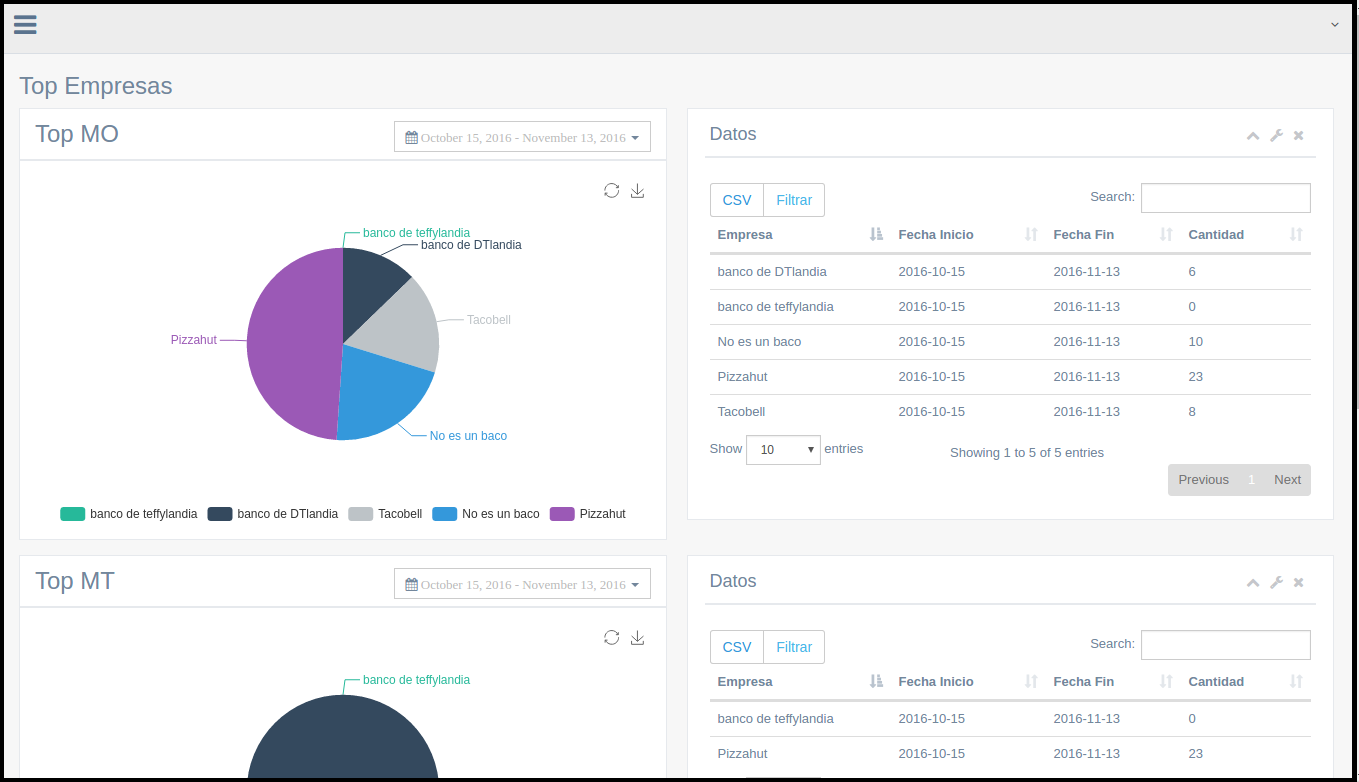
\includegraphics[scale=0.30,type=png,ext=.png,read=.png]{imagenes/rete}
  \caption{Reporte Empresa: Top Empresa.}
  \label{fig:rete}
\end{figure}

% \pagebreak


\indent En este \textit{Sprint} se procedió de manera similar al anterior, primero se desarrollaron los servicios REST para la obtención de datos para ambos reportes y luego se integraron cada uno con sus respectivos graficos y tablas. Finalmente se integraron los \textit{widget} calendario en cada reporte.


\subsubsection{Desarrollo de vistas Campañas y Distribución Operadoras}
\indent La vista \textit{Campañas} muestra todas las campañas de mensajerías asociadas a la empresa a la cual pertenece el usuario. Como se puede observar en la figura \ref{fig:campana}, es una tabla que muestra la información pertinente de las campañas de la empresa, proveniente de la llamada a un servicio REST.
\begin{figure}[ht]
  \centering
  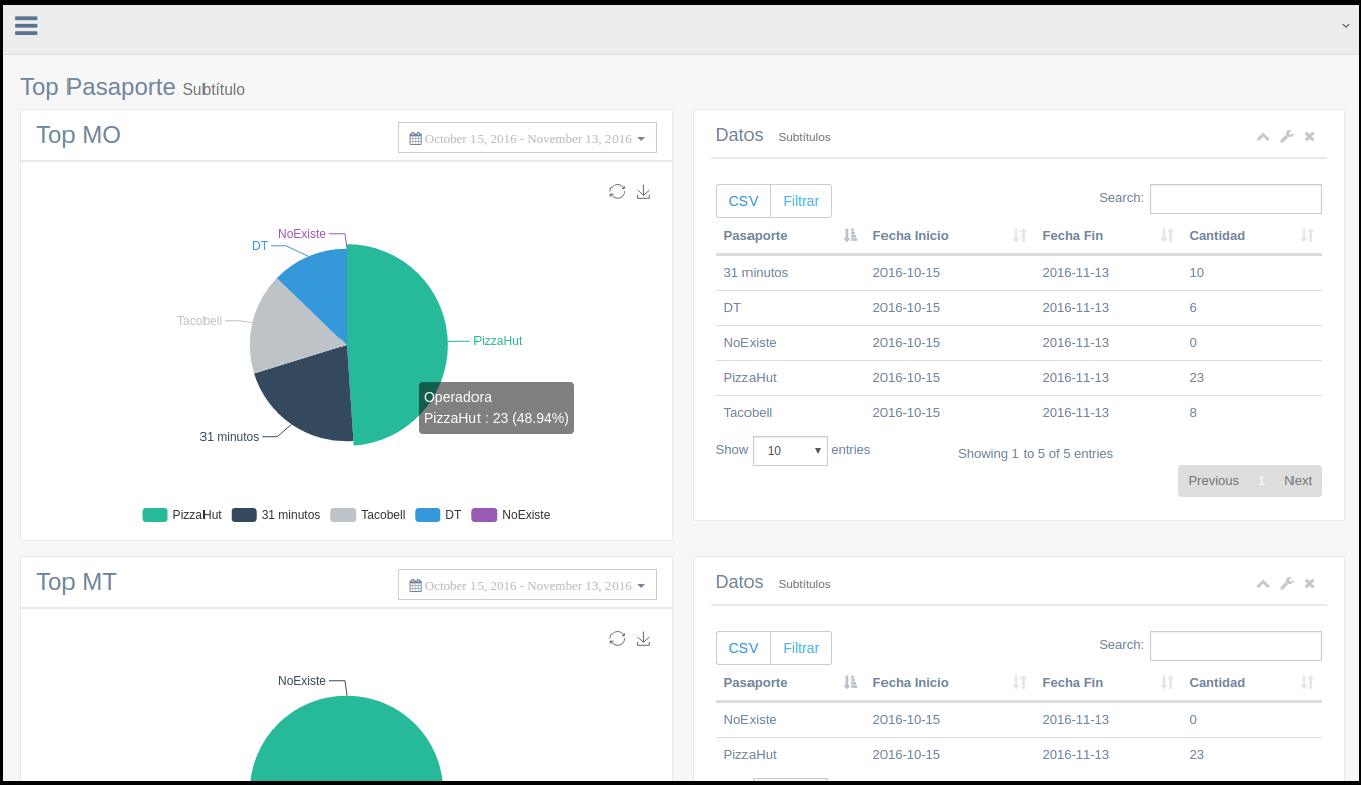
\includegraphics[scale=0.30,type=png,ext=.png,read=.png]{imagenes/retp}
  \caption{Reporte Empresa: Top Pasaporte.}
  \label{fig:retp}
\end{figure}
\newline
\newline
\indent Miestras que \textit{Distribución Operadoras} es un reporte parecido a \textit{Top Empresas}, donde se muestra la cantidad de mensejes enviados por cada operadora asociada a dicha empresa. El reporte de la distribución de las operadoras esta divido en tres secciones MO, MT e Interactivos, de igual menera que los repotes de \textit{Top Empresa} y \textit{Top Pasaportes}.
\begin{figure}[ht]
  \centering
  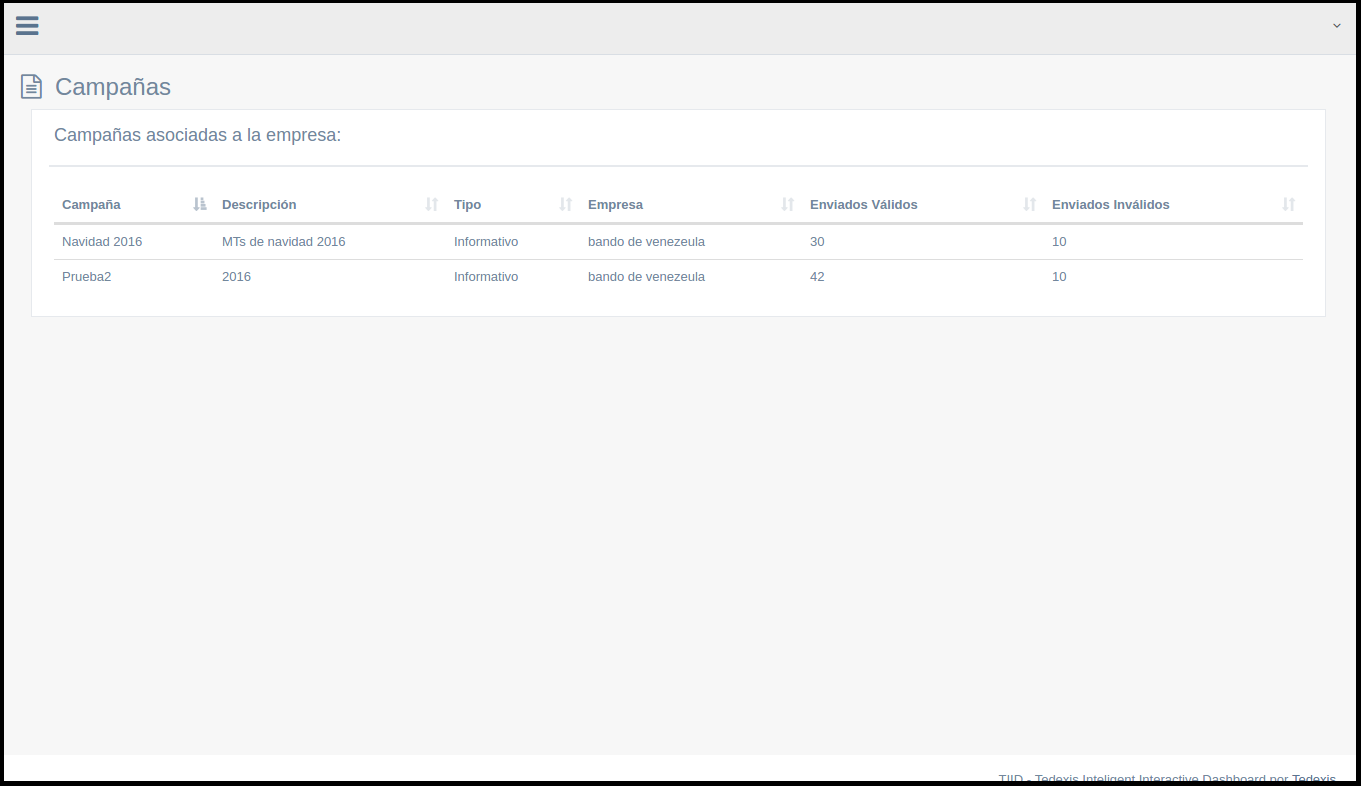
\includegraphics[scale=0.30,type=png,ext=.png,read=.png]{imagenes/campana}
  \caption{Reporte Empresa: Campañas.}
  \label{fig:campana}
\end{figure}

\subsubsection{Pruebas}
\indent Las pruebas realizadas en este \textit{Sprint} se realizaron de manera similar que las anteriores. Primero se realizaron pruebas unitarias a cada servicio REST y luego se integraron con lo desarrollado en el front-end. En este caso se tuvieron algunas dificultades en principio con el desarrollo de \textit{Top Empresas}, debido a que es una vista con más de una tabla y más de un gráfico por lo que se gneraban algunos conflictos de superposición de gráfico y ciertos filtros no ejercían su función en la tabla correspondiente. Esto se solucionó creando un controlador diferente por cada conjunto gráfico-tabla de cada reporte, es decir, en el caso de \textit{Top Empresas} se crearon 3 controladores diferentes, uno para \textit{Top MO}, otro para \textit{Top MT} y otro para \textit{Top Interactivos}. Esta misma lógica fue aplicada en los reportes \textit{Top Pasaportes} y \textit{Distribución Operadoras}.  

% %%%%%%%%%%%%%%%%%%%%%%%%%%%%

\section{Desarrollo de Reportes por Pasaporte} \label{sect:Desarrollo de Reportes por Pasaporte}

\subsection{Objetivos}
\begin{itemize}[noitemsep,nolistsep]
\item Desarrollo de reportes por pasaporte. 
\end{itemize}

\subsection{Actividades}

\subsubsection{Desarrollo de vistas de reporte de tráfico}
\indent Se inició desarrolando las vista \textit{Evolución del Tráfico} para el reporte por pasasporte. Este reporte es similar al realizado anteriormente en los reportes por empresa, con la diferencia que primero se debe elegir un pasaporte del usuario en sesión, mostrados en una tabla al incio de la vista, y luego se muestra el tráfico de dicho pasaporte, como se puede observar en la figura \ref{fig:rpet}.
\pagebreak
\begin{figure}[ht]
  \centering
  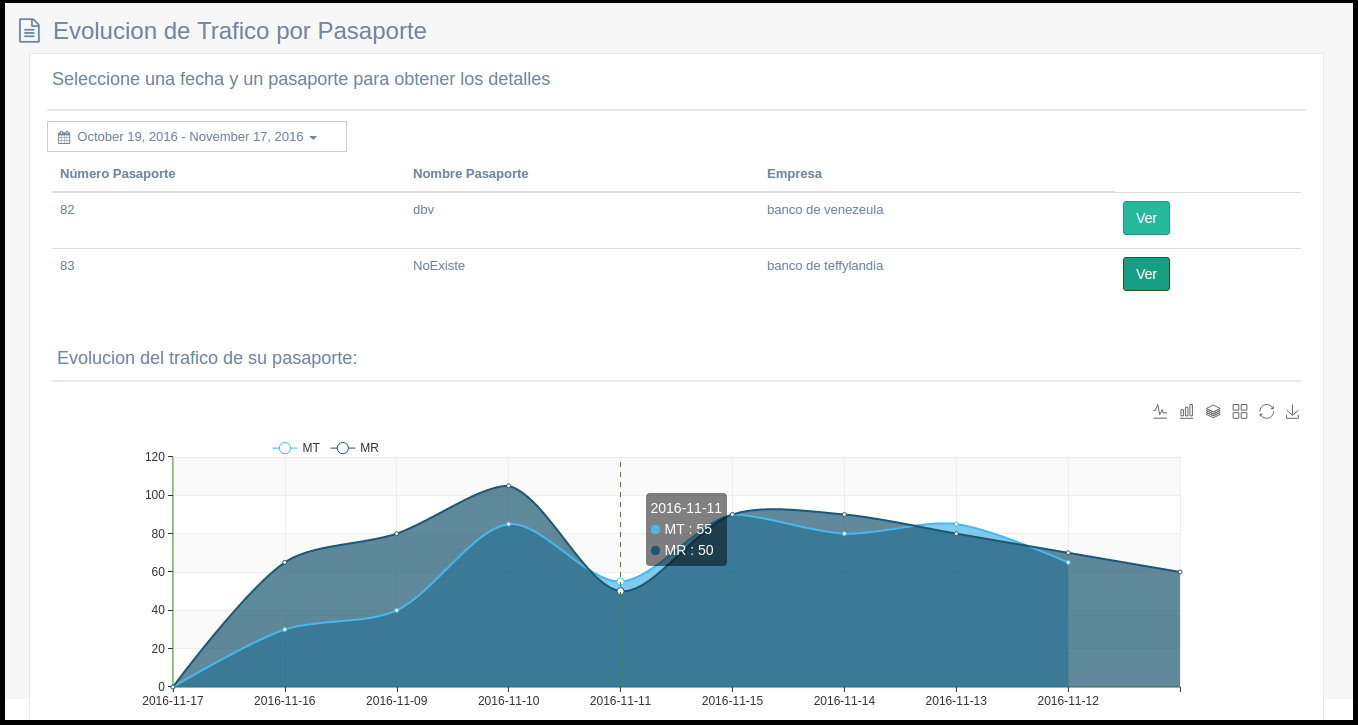
\includegraphics[scale=0.30,type=png,ext=.png,read=.png]{imagenes/rpet}
  \caption{Reporte Pasaporte: Evolución del Tráfico.}
  \label{fig:rpet}
\end{figure}

\indent La información mostrada en los reportes \textit{Evolución del Tráfico}, \textit{Evolución Día} y \textit{Evolución Hora} son análogos a sus versiones en el apartado \textit{Reporte Empresa}, correspondiendo a tráfico de mensajes por día de los tipos MT y MR para \textit{Evolución del Tráfico} y de los tipos MO y MT para \textit{Evolución Día}, mostrado en la figura \ref{fig:rped}, mientras que \textit{Evolución Hora} al seleccionar un pasaporte, muestra el tráfico por hora de los mensajes tipo MT y MO, como se observa en al figura \ref{fig:rpeh}.

\begin{figure}[ht]
  \centering
  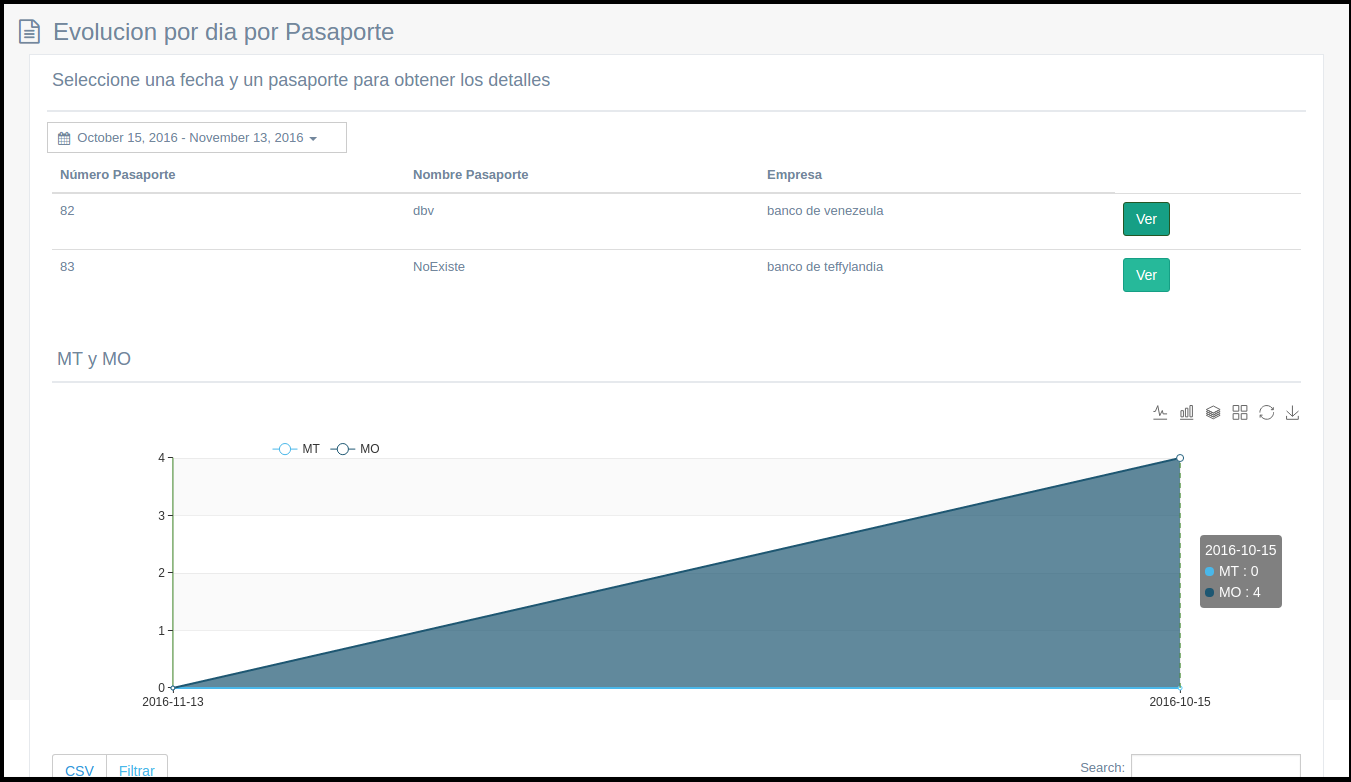
\includegraphics[scale=0.30,type=png,ext=.png,read=.png]{imagenes/rped}
  \caption{Reporte Pasaporte: Evolución Día.}
  \label{fig:rped}
\end{figure}

\begin{figure}[ht]
  \centering
  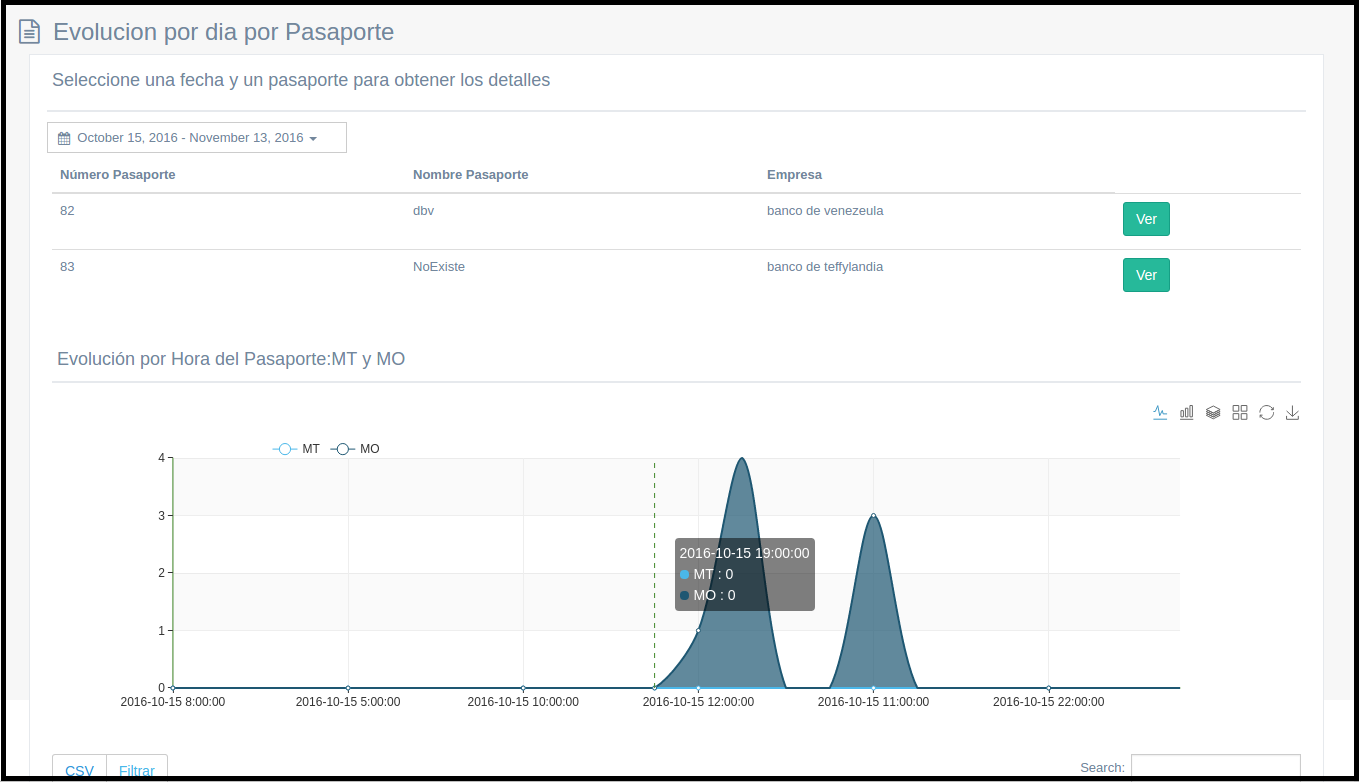
\includegraphics[scale=0.30,type=png,ext=.png,read=.png]{imagenes/rpeh}
  \caption{Reporte Pasaporte: Evolución Hora.}
  \label{fig:rpeh}
\end{figure}

\indent Para el desarrollo de estas vistas, se tomaron como base los servicios REST creados para los reportes por empresa, los cuales fueron adaptados para que hicieran las consultadas a las colecciones consolidadas en base, utilizando los pasaportes en vez de las empresas. De igual manera, para el front-end se tomaron como plantillas las vistas de los reportes por empresa, se le agregaron una tabla nueva donde muestran los pasaportes pertenecientes al usuario y se crearon las funcionalidades pertinentes para integración de todo. No resultó ningún inconveniente en el desarrollo.
\newline
\newline
\indent El desarrollo de \textit{Distribución Operadoras} se realizó de manera similar a lo expuesto anterior mente, se tomaron el servicio REST y la plantilla de la vista del reporte \textit{Distribución Operadora} por empresa y fueron adaptados de la misma forma. En el servicio REST fueron modificadas las consultas ya no por empresa sino por pasaporte y a la vista se le agregó una nueva tabla donde se elige un pasaporte y se muestra el reporte de la distribución de mensajes, enviados por dicho pasaporte, por operadora.

\subsubsection{Pruebas}
\indent Las pruebas se iniciaron con pruebas unitarias a los nuevos servicios REST desarrollados, verificando que las consultas estuvieran siendo realizadas en base al pasaporte suministrado y no en base a la empresa. Seguidamente, se realizaron pruebas de integración de las nuevas tablas que contienen todos los pasaportes asociados a un usuario y verificando que la información mostrada por pantalla, fueran los reportes pertenecientes al pasaporte seleccionado anteriorme. No resultaron ningún inconveniente en estas pruebas. De igual manera, las pruebas fueron mostradas y aprobadas por el \textit{Product Owner} y el \textit{Scrum Master}.

% %%%%%%%%%%%%%%%%%%%%%%%%%%%%

\section{Desarrollo de ultimas vistas del front-end} \label{sect:Desarrollo de ultimas vistas del front-end}

\subsection{Objetivos}
\begin{itemize}[noitemsep,nolistsep]
\item Desarrollo la vista principal y soporte. 
\end{itemize}

\subsection{Actividades}
\indent Con este \textit{Sprint} se finalizó el desarrollo del sistema, antes de ser montado en un servidor local dentro de Tedexis para que fuera probado por el personal de la empresa.

\subsubsection{Vista principal}
\indent Para la vista principal se solicitó que tuviera un resumen de los reportes por empresa asociado al usuario, mostrando directamente distintos gráficos y la cantidad de mensajes enviados por ese usuario en el mes en curso. Ya que se deseaba que el usuario pudiera visualizar directamente información pertinente desde su entrada al sistema. Como se puede observar en la figura \ref{fig:principal}. Dichos requerimientos fueron cumplidos utilizando los servicios REST creados durante el desarrollo, al igual que las mismas funciones para la creación de gráficos. 

\begin{figure}[ht]
  \centering
  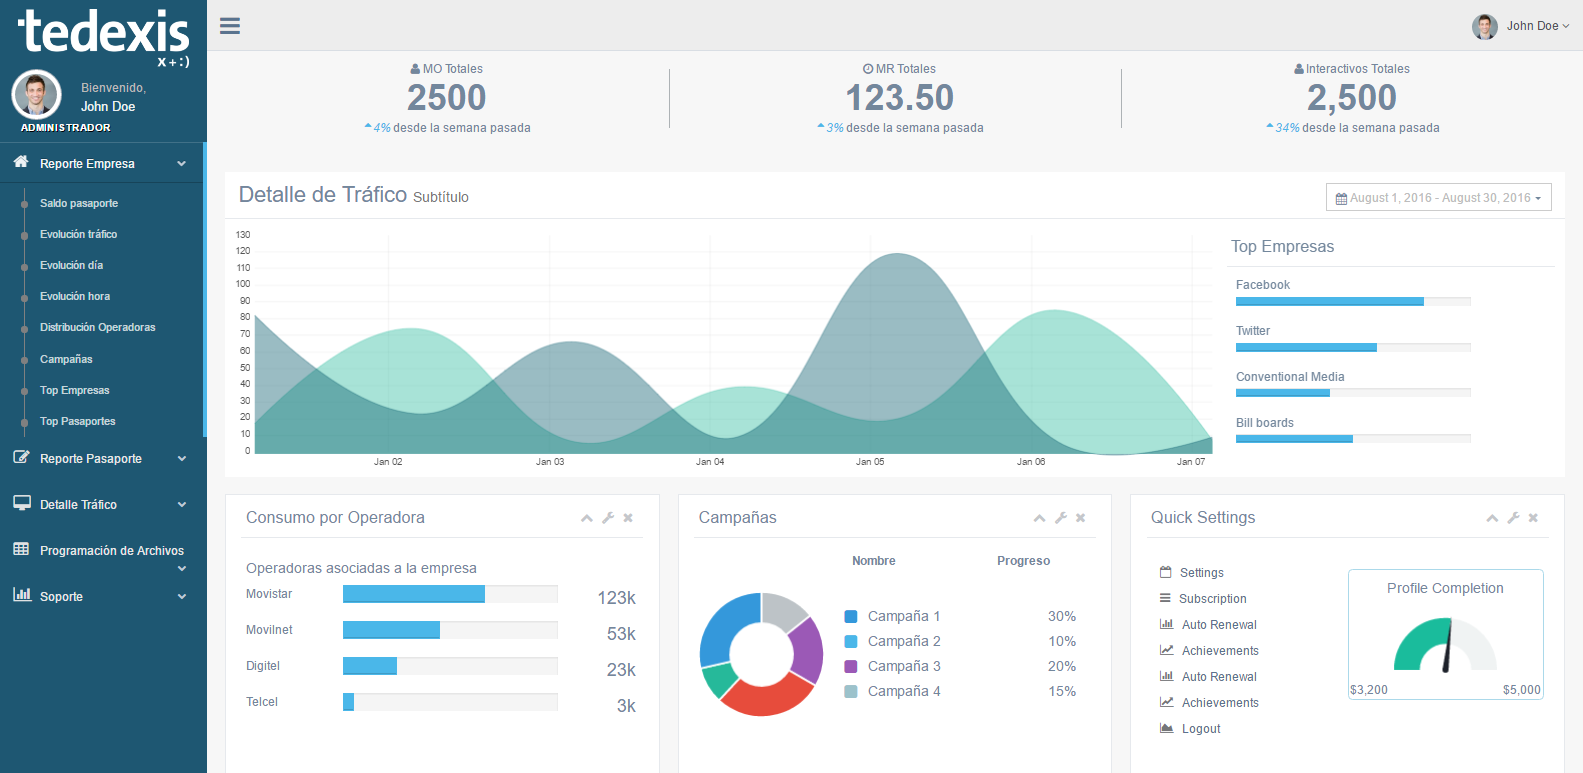
\includegraphics[scale=0.30,type=png,ext=.png,read=.png]{imagenes/principal}
  \caption{Vista principal.}
  \label{fig:principal}
\end{figure}

\subsubsection{Soporte}
\indent El apartado de soporte se posee un formulario llamado \textit{Generar ticket}, el cual al ser completado con la información requerida, envía un correo al Departamento de Soporte de Tedexis para la gestión de la solicitud del cliente. Se puede visualizar esta vista en la figura \ref{fig:soporte}.

\begin{figure}[ht]
  \centering
  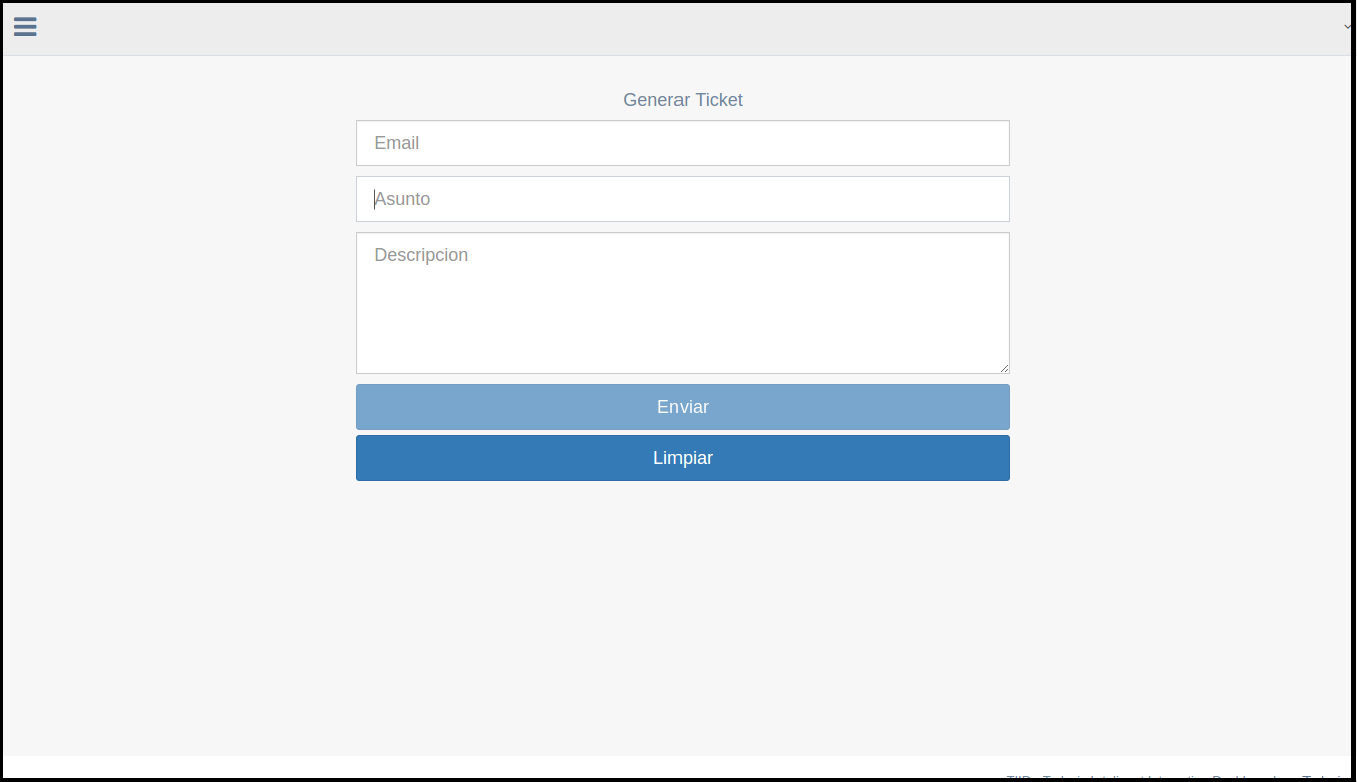
\includegraphics[scale=0.30,type=png,ext=.png,read=.png]{imagenes/soporte}
  \caption{Vista soporte.}
  \label{fig:soporte}
\end{figure}

% %%%%%%%%%%%%%%%%%%%%%%%%%%%%

\section{Pruebas por el personal de la empresa} \label{sect:Pruebas por el personal de la empresa}

\subsection{Objetivos}
\begin{itemize}[noitemsep,nolistsep]
\item Pruebas y certificación. 
\end{itemize}

\subsection{Actividades}

\subsubsection{Pruebas del equipo de producto}

\indent A medida que se fueron realizando los sprint de desarrollo, se fueron realizando pruebas unitarias y de integración tanto en el front-end, como en el back-end y en los servicios rest, dependiendo de lo desarrollado en el sprint.
\newline
\newline
\indent Posteriormente, el \textit{Scrum Master} decidió montar localmente en un servidor de la empresa el sistema realizado con el fin de recibir mayor retroalimentación por parte del personal de Tedexis. Inicialmente fue probador por el equipo del Departamento de Producto (los que desarrollan las aplicaciones dentro de la empresa), quienes se enfocaron mayormente en el código realizado, proveyendo recomendaciones de refactorización y documentación del código, especificamente en el back-end y en los servicios rest. De igual manera, propusieron ideas para la optimización de consultas de bases de datos de MongoDB, donde se utilizaron expresiones regulares y métodos de agrupación proporsionados por dicho manejador.

\subsubsection{Pruebas del equipo de comercio}

\indent Seguidamente de las pruebas realizadas por el Departamento de Producto, se les informó al Departamente de Comercio que podían ingresar al sistema y realizaran las pruebas pertinentes. La opinión de este departamento es sumamente importante debido a que son quienes más utilizarían el sistema, además de ser quien lo vende a los clientes de la empresa.
\newline
\newline
\indent Las observaciones por parte de este departamento fueron en su mayoría enfocadas en el fron-end del sistema, solicitando cambios en la paleta de colores utilizada, la cual ayudaría a asociar al cliente con la empresa de forma más visual y directa; solicitud de que la información exportada de los diferentes reportes solo fuera en formato csv; solicitud de poder descargar los gráficos mostrados en los diferentes repotes en forma de imagenes; solicitud de poder cambiar entre gráfica de barra y gráfica de puntos en los reportes de tráfico de mensajes.

% %%%%%%%%%%%%%%%%%%%%%%%%%%%%

\section{Redacción del libro de pasantía} \label{sect:Redaccion del libro de pasantia}

\subsection{Objetivos}
\begin{itemize}[noitemsep,nolistsep]
\item Redacción de libro de pasantía. 
\end{itemize}

\subsection{Actividades}

\subsubsection{Redacción del libro y versión final de los documentos de la empresa}
\indent Como fue propuesto en el plan de trabajo, las últimas dos semanas fueron dedicadas a la redacción del libro de pasantías, adicinalmente, se actualizaron los documentos solicitados por la empresa, que pueden ser encontrados en los apendices.

% %%%%%%%%%%%%%%%%%%%%%%%%%%%%



\chapter{Conclusiones y Recomendaciones} \label{chapter:Conclusiones y Recomendaciones}

Al culminar el tiempo estipulado para el desarrollo de la pasantía, se puede afirmar que los objetivos inciales fueron alcanzados en su mayoría y superados en muchos casos, obteniendo un producto final que satisface las necesidades tanto de los clientes como el personal de la empresa que hace uso del sistema.
\newline
\newline
\indent La versión TIID supera en velocidad de acceso y respuesta a su versión anterior TID. El nuevo sistema posee una interfaz gráfica agradable y cómoda para el usuario, quien tiene acceso a una diversidad de reportes relevantes que lo mantienen al tanto de su actividad con la empresa. Dichos reportes estan divididos en dos apartados: Reportes por Empresa, donde se muestran distintos reportes basados en la información provenientes de todos los clientes asociados a la empresa del usuario; y Reportes por Pasaporte, donde se muestran en detalle distintos resportes referentes a cada pasasporte asociado al usuario. Los reportes mencionados poseen distintos mecanismos de búsqueda y filtros para su mejor visualización, de igual manera, pueden ser exportados si el usuario lo desea.
\newline
\newline
\indent TIID se divide en back-end, front-end y servicios web, donde el back-end se encarga de la consolidación de los mensajes enviados por la plataforma Mercurio en un día, realizado por dos hilos: uno que consolida los mensajes enviados por día y otro que lo hace por hora, esto se almacena en una base de datos NoSQL. Dicha consolidación se lleva acabo para el rápido acceso de información en las consultas realizadas por los servicios web, que en este caso fueron implementados siguiendo la aquitectura REST, quienes proveen los datos consultados en formato tipo JSON. Finalmente dicha información es desplegada en el front-end del sistema como reportes en forma de gráficas y tablas de datos, los cuales pueden ser consultados en diferentes rangos de tiempo y descargados si el usuario lo desea.
\newline
\newline
\indent En cuanto a la metodología de desarollo se puede afirmar, que \textit{Scrum} resultó ser un buen mecanismo de desarrollo, permitiendo que se realizara de manera organizada, manteniendo constante comunicación con el \textit{Product Owner} y el \textit{Scrum Master} y sobre todo, la rápida y fluida adaptación durante el desarrollo a cambios, sugerencias e improvistos surgidos.
\newline
\newline
\indent Como recomendaciones para la empresa se puede mencionar: mejorar la comunicación entre los Departamentos Comercio, Producto y Operaciones, ya que muchas veces proveían diferente información sobre un mismo requerimiento del producto, por lo que había que invertir tiempo adicional en definir nuevamente los puntos y llegar a nuevos acuerdos; disposición a utilizar nuevas tecnologías, debido a que todo lo desarrollan utilizando java y están un poco cerrados a probar diferentes tecnologías que les pueden llegar a ser muy útiles; y realizar y mantener organizada documentación relevante de los productos desarrollados por la empresa.
\newline
\newline
\indent Esta experiencia sirvió para integrar al pasante en un ambiente laboral real, donde se le permitió un diseñar y desarrollar un producto que resuelve una problemática que sufre actualmente la empresa. Integrarlo en una situación donde el trabajo en equípo y la comunicación fueron pilares fundamentales para el logro de las metas propuestas. De igual manera, permitió al pasante indagar y aprender nuevas tecnologías y herramientas utilizadas en producción por muchas compañías. Una experiencia integra, que permitió el desarrollo tanto personal como profesional.
\newline
\newline
\indent Finalmente, queda como trabajo futuro el desarrollo a fondo del módulo de autenticación del sistema, desarrolando una mayor cantidad de perfiles y toda la lógica que conlleva y la integración de otros dos sistemas como módulos dentros de TIID, dichos sistemas son: Reporte del tráfico detallado (RTD) y el sistema de programación de envío masivo de mensajes (TrinityKronos), los cuales no fueron desarrollados en este proyecto de pasantias.


% Establece las citas y bibliografia
\bibliographystyle{ieeetr}
\bibliography{referencias}

%\glsaddall
%\printglossary

% Crea el apendice
\appendix
\chapter{Documento de Definición de Requerimientos }
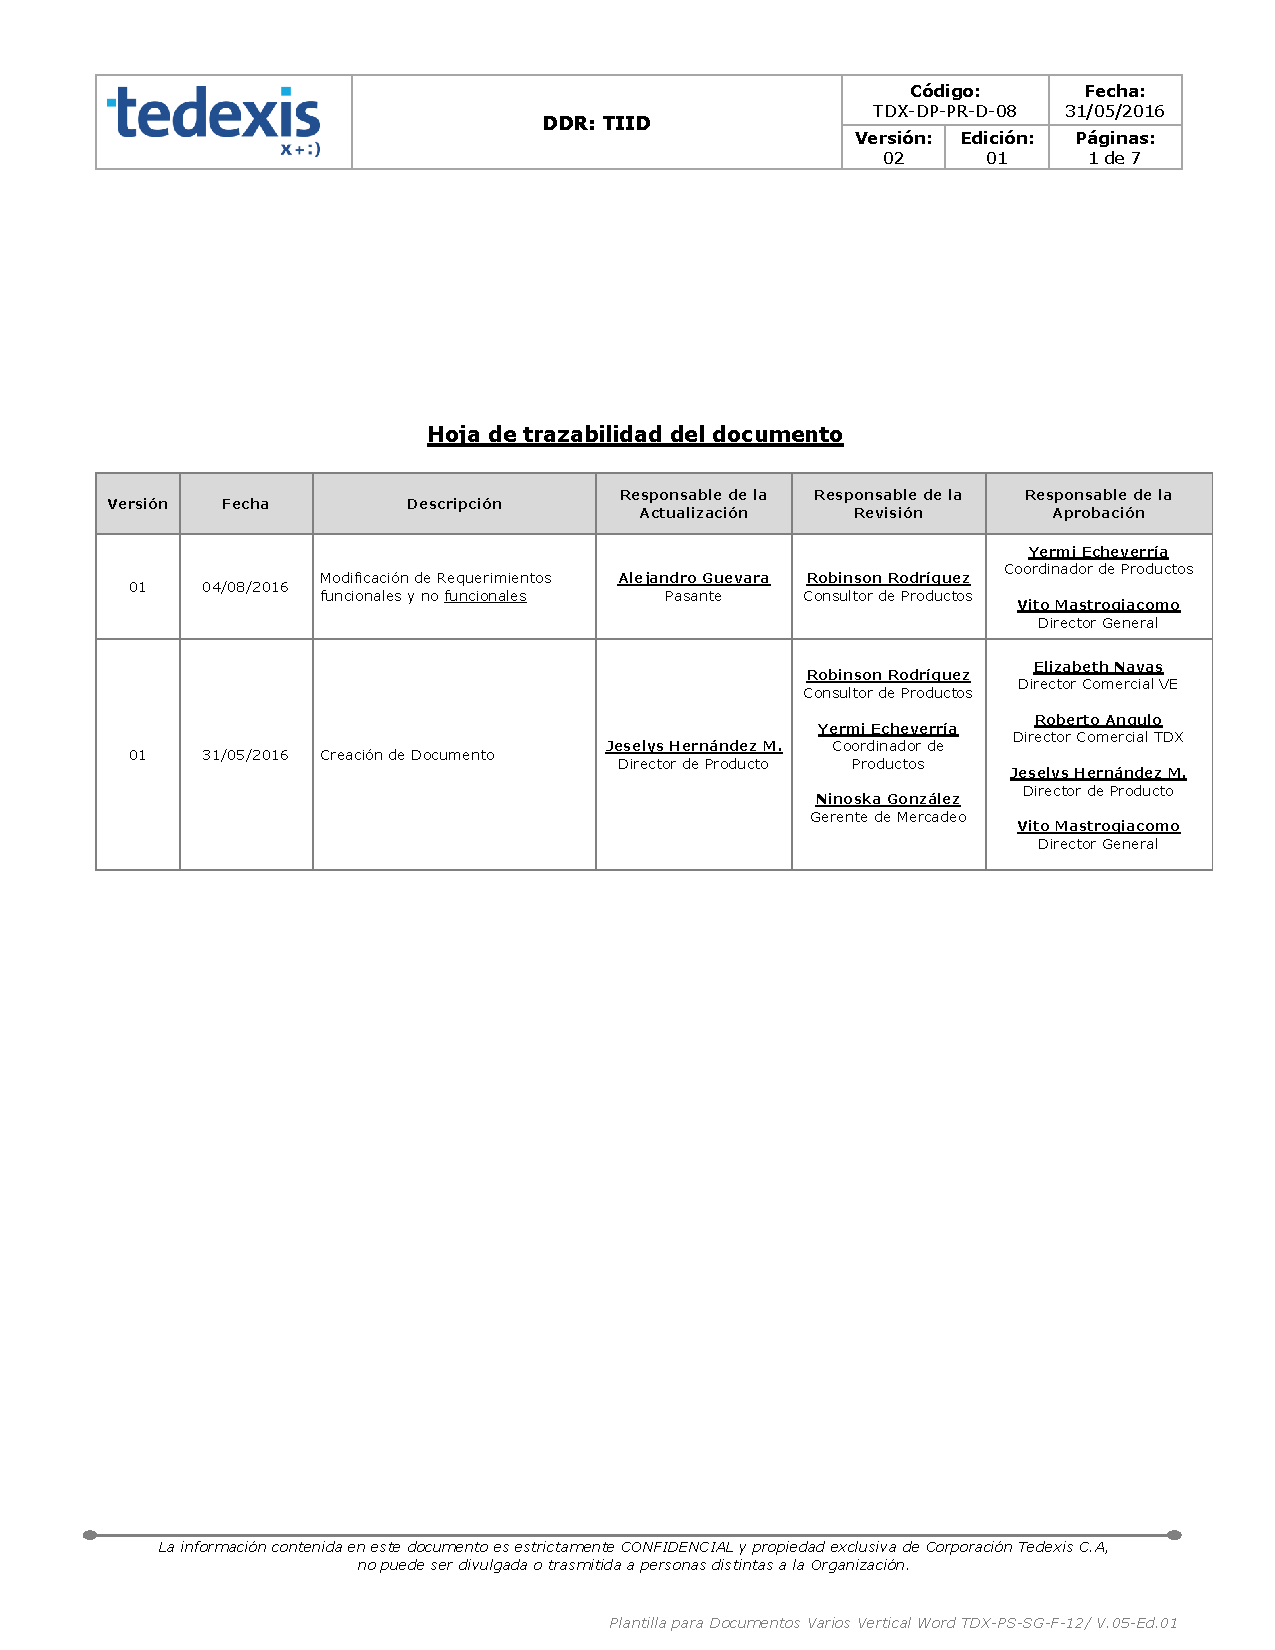
\includepdf[pages=-]{apendices/TDXDPPRD08DDRTIID.pdf}
\chapter{Documento de Definición de Proyecto }
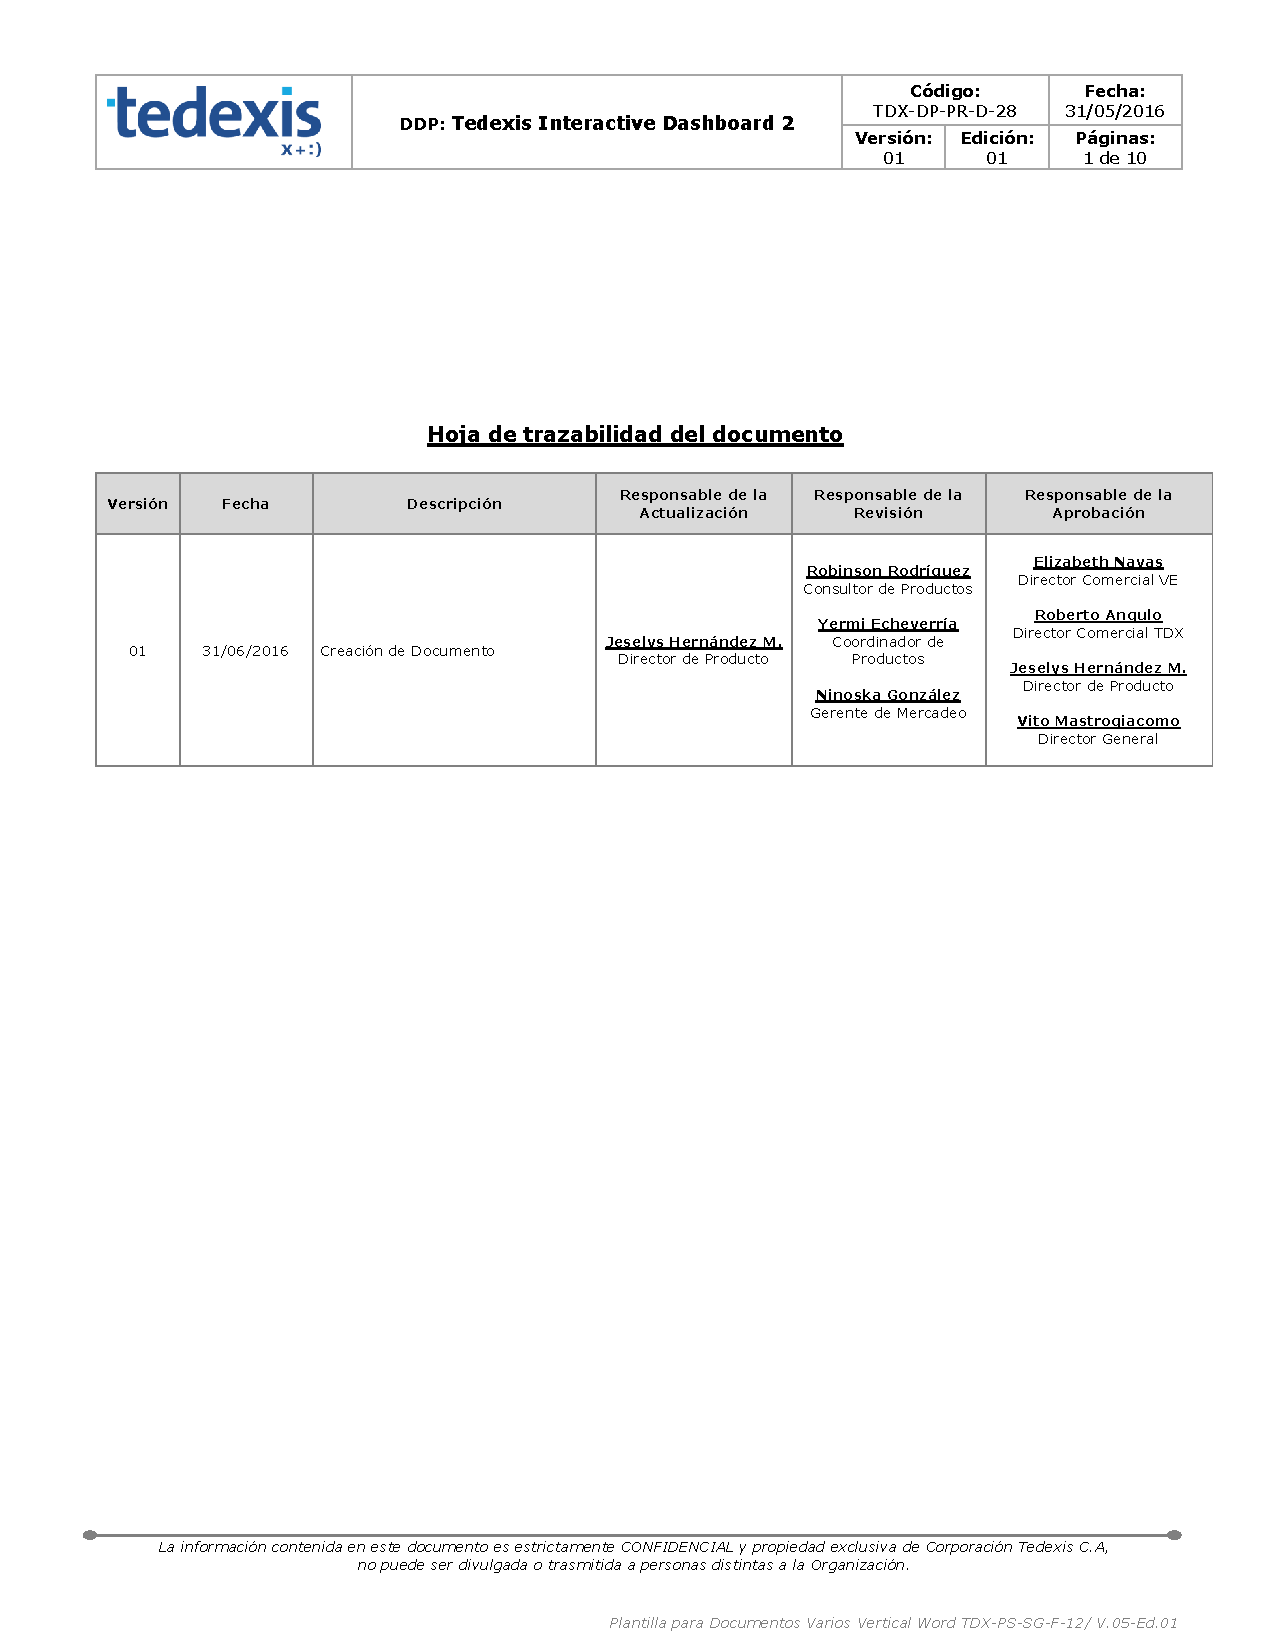
\includepdf[pages=-]{apendices/TDXDPPRD28DDPTIID.pdf}
%\chapter{Manual de Usuarios de NetPass}
%\includepdf[pages=-]{apendices/ManualUSUARIOS.pdf}
%\chapter{Especificación de servicios del Asistente para ensamblar aplicaciones móviles}
%\includepdf[pages=-]{apendices/PortadaServicios.pdf}
%\includepdf[pages=-]{apendices/Kiraso_services.pdf}
%\chapter{Matriz de pruebas}
%\includepdf[pages=-]{apendices/PortadaPruebas.pdf}
%\includepdf[pages=-14]{apendices/pruebas-kiraso.pdf}
%\chapter{Manual Kiraso}
%\includepdf[pages=-]{apendices/PortadaManual.pdf}
%\includepdf[pages=-]{apendices/ManualKiraso.pdf}

\end{document}
